%%%%%%%%%%%%%%%%%%%%%%%%%%%%%%%%%%%%%%%%%%%%%%%%%%%%%%
% THE LM WIMDP POWER BEAMER CLASS
% (example document)
%
% Carlos Arce <caar@lmwindpower.com>
% November, 2011
%
% Description:
%	This document contains most if not all the elements
%	that will likely be used in a presentation. Other
%	elements, and details on how to manipulate the 
%	ones herein presented are detailed in the Beamer
%	Class User Guide (google it).
%
%%%%%%%%%%%%%%%%%%%%%%%%%%%%%%%%%%%%%%%%%%%%%%%%%%%%%%


%Everything starts like this
%But add the xcolot=table option if you want colored tables
\pdfminorversion=4
\documentclass[xcolor=table,aspectratio=169]{beamer}
\usepackage[english]{babel}
\usepackage{natbib}
\usepackage[squaren]{SIunits}
\usepackage{media9}
\usepackage{booktabs}
\usepackage{multicol}
\usepackage{multirow}
\usepackage{multimedia}
\let\mathrm\mathsf
% make bibliography entries smaller
\renewcommand\bibfont{\scriptsize}
% If you have more than one page of references, you want to tell beamer
% to put the continuation section label from the second slide onwards
\setbeamertemplate{frametitle continuation}[from second]
% Now get rid of all the colours
\setbeamercolor*{bibliography entry title}{fg=black}
\setbeamercolor*{bibliography entry author}{fg=black}
\setbeamercolor*{bibliography entry location}{fg=black}
\setbeamercolor*{bibliography entry note}{fg=black}
% and kill the abominable icon
\setbeamertemplate{bibliography item}{}

\newcommand\blfootnote[1]{%
  \begingroup
  \renewcommand\thefootnote{}\footnote{#1}%
  \addtocounter{footnote}{-1}%
  \endgroup
}

% beamer: How to place images behind text (z-order)
% (http://tex.stackexchange.com/a/134311)
\makeatletter
\newbox\@backgroundblock
\newenvironment{backgroundblock}[2]{%
  \global\setbox\@backgroundblock=\vbox\bgroup%
    \unvbox\@backgroundblock%
    \vbox to0pt\bgroup\vskip#2\hbox to0pt\bgroup\hskip#1\relax%
}{\egroup\egroup\egroup}
\addtobeamertemplate{background}{\box\@backgroundblock}{}
\makeatother

%\setbeamertemplate{bibliography item}[text]
%Of course, the LM beamer class call:
\usetheme{LM}

%Any other packages should go here

%And the begin document environment as usual
\begin{document}

%%%%%%%%%%%%%%%%%%%%%%%%%%%%%%%%%%%%%%%%%%%%%%%%%%%%%%
% The owner information
%%%%%%%%%%%%%%%%%%%%%%%%%%%%%%%%%%%%%%%%%%%%%%%%%%%%%%

%The title (short title in square brackets)
\title[Flow-misaligned Serrations]{Effects of Serration-Flow Misalignment}

%The author (short author in square brackets, although not used)
\author[Carlos Arce Le\'on]{Carlos Arce Le\'on}

%The date (put \today to insert today's date automatically)
\date{October 18, 2016, Leiden\\Serration Technology on Airfoil} 

%The owner's job title at LM (for the contact information)
\jobtitle{Senior Engineer}

%The owner's department
\department{Aerodynamics and Acoustics}

%The owner's fixed line phone number (optional)
\phone{+31 725 752 020}

%The owner's mobile phone number (optional)
\mobile{+31 642 652 145}

%The owner's email (optional)
\email{caar@lmwindpower.com}


%%%%%%%%%%%%%%%%%%%%%%%%%%%%%%%%%%%%%%%%%%%%%%%%%%%%%%
% The front matter
%%%%%%%%%%%%%%%%%%%%%%%%%%%%%%%%%%%%%%%%%%%%%%%%%%%%%%

%The title page (remember to use the option plain!)
\frame[plain]{
\titlepage
} 

%Include an LM style formatted table of contents
\Agenda

%%%%%%%%%%%%%%%%%%%%%%%%%%%%%%%%%%%%%%%%%%%%%%%%%%%%%%
% The body of the presentation
%%%%%%%%%%%%%%%%%%%%%%%%%%%%%%%%%%%%%%%%%%%%%%%%%%%%%%
% - Use sections and subsections wisely
%
\section{Introduction}

\begin{frame}[c]{LM Wind Power}{who we are and what we do}
    \begin{backgroundblock}{-0.1mm}{65mm}
        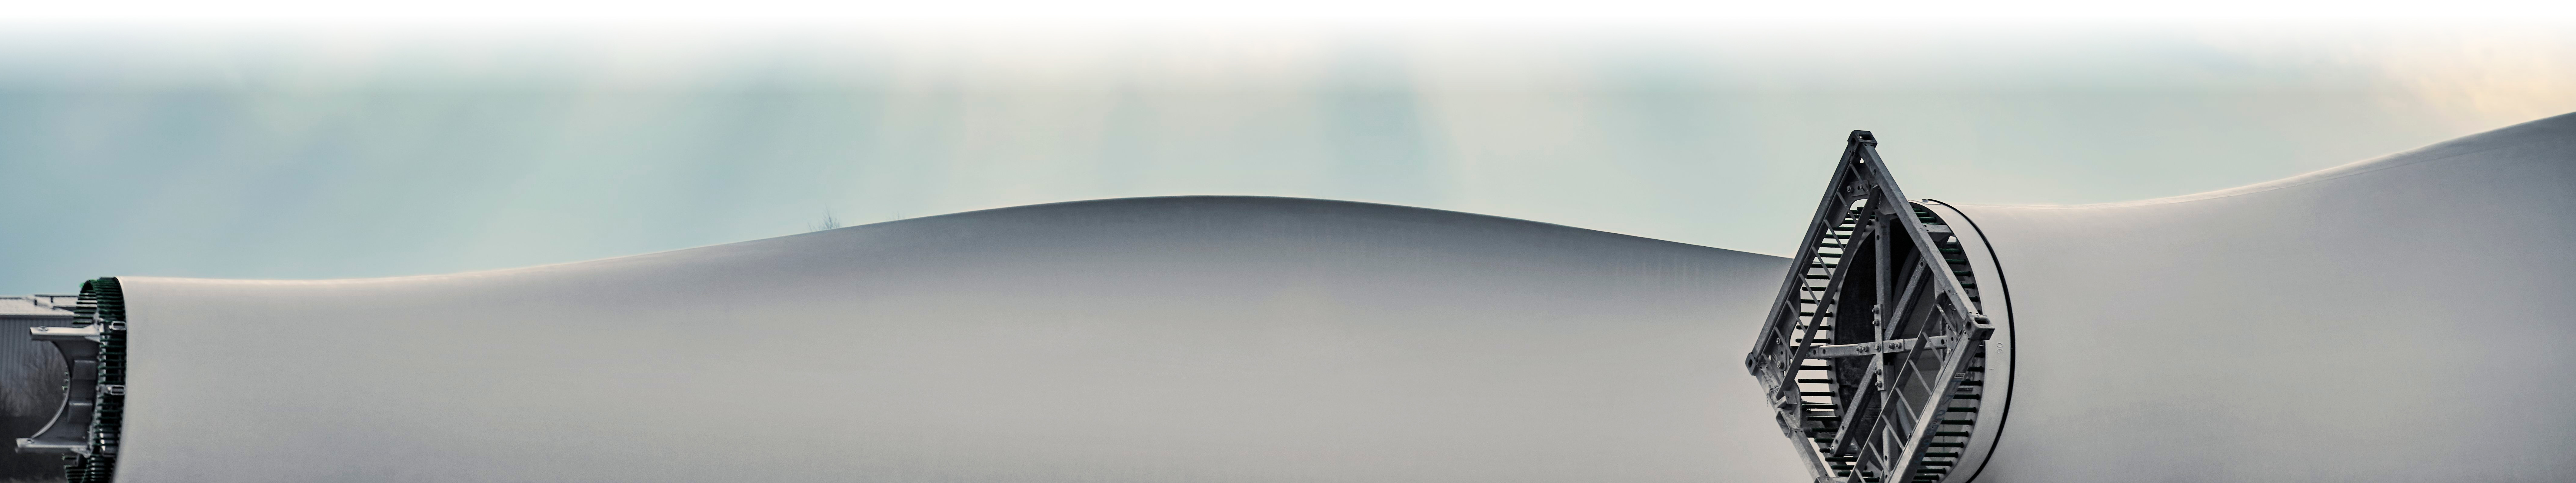
\includegraphics[width=1.2\textwidth]{media/bottom.jpg} 
    \end{backgroundblock}
    \begin{columns}
        \column{0.4\textwidth}
        \scriptsize{
        \vspace{1cm}
        \begin{itemize}
            \item Over $8178$ employees (end 2016)
            \item in 14 factories around the world
            \item and 3 engineering centers
        \end{itemize}
        \vspace{5mm}
        \begin{itemize}
            \item 1 out of 5 turbines use our blades
            \item $\unit{84}{\giga\watt}$ installed capacity
            \item we've helped mitigate $166$ million metric tons of CO$^2$
        \end{itemize}
    }
        \column{0.6\textwidth}
        \vspace{1cm}
        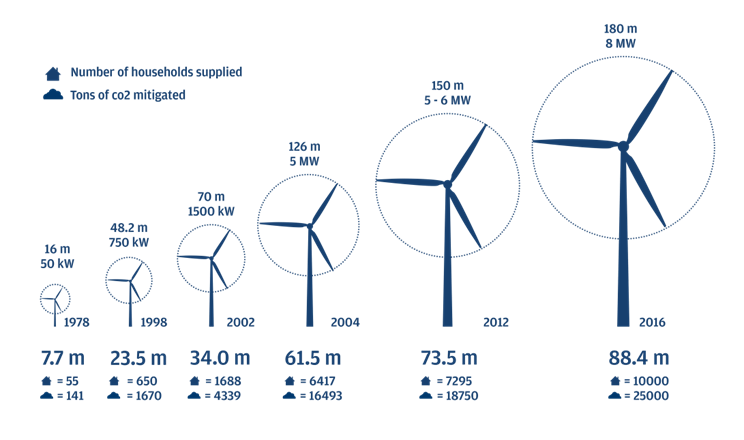
\includegraphics[width=\textwidth]{media/LMRotors.png}
    \end{columns}
    \blfootnote{\textcolor{white}{Calculations based on European data}}
\end{frame}

{
\setbeamercolor{background canvas}{bg=black}
\begin{frame}[plain,c]
    \vspace{-2mm}
    \begin{backgroundblock}{1cm}{0mm}
        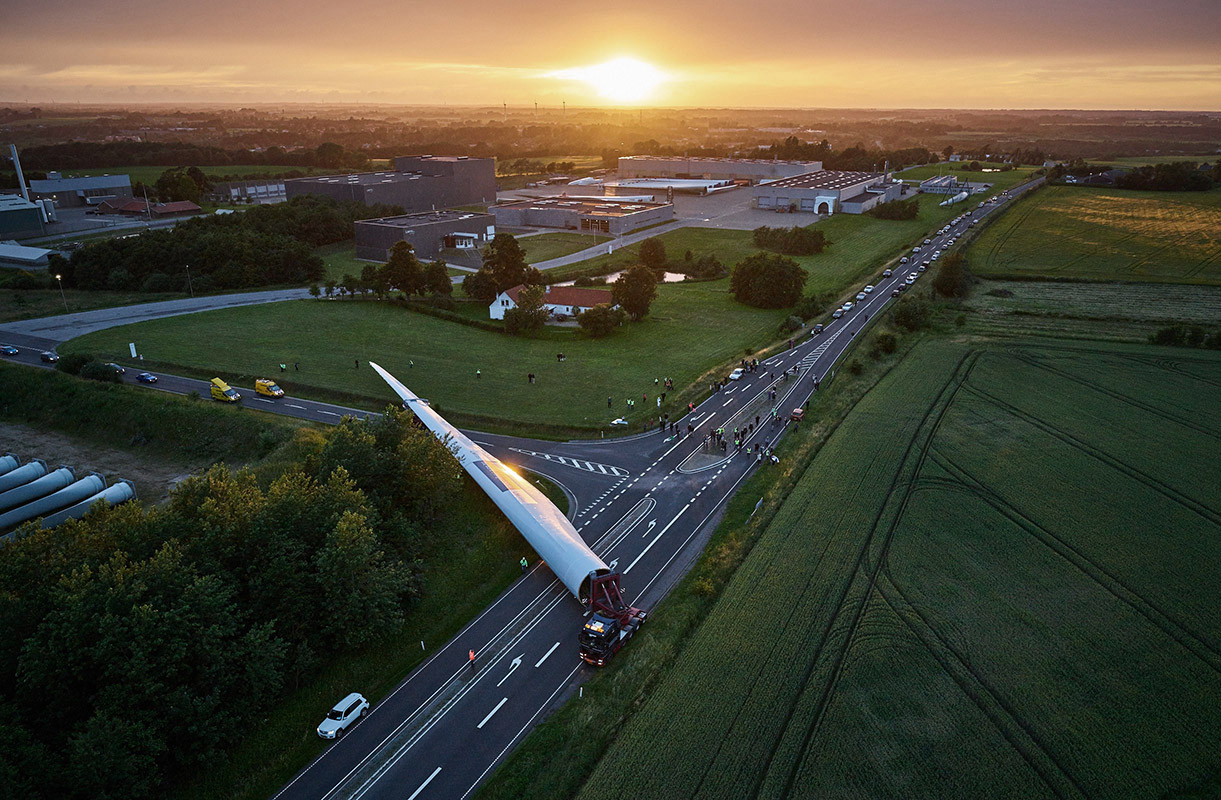
\includegraphics[width=1.0\textwidth]{media/88Transport.jpg} 
    \end{backgroundblock}
    \vspace{-2cm}\hspace{8.5cm}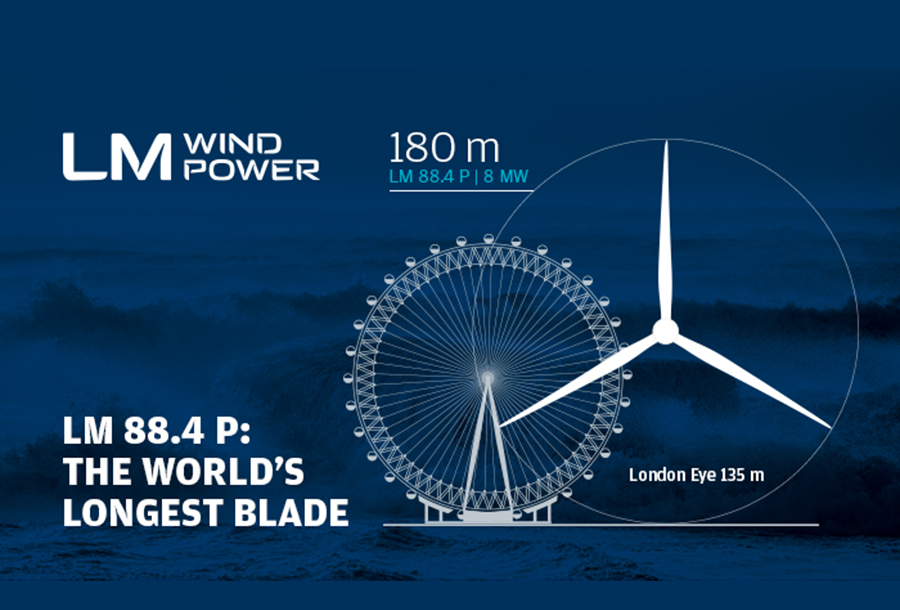
\includegraphics[width=0.35\textwidth]{media/88comparison.jpg}
\end{frame}
}

\begin{frame}{}{}
    \Large \bf \textcolor{LMLightBlue}{Trailing edge serrations \\in the wind industry}
    \begin{backgroundblock}{70mm}{0mm}
        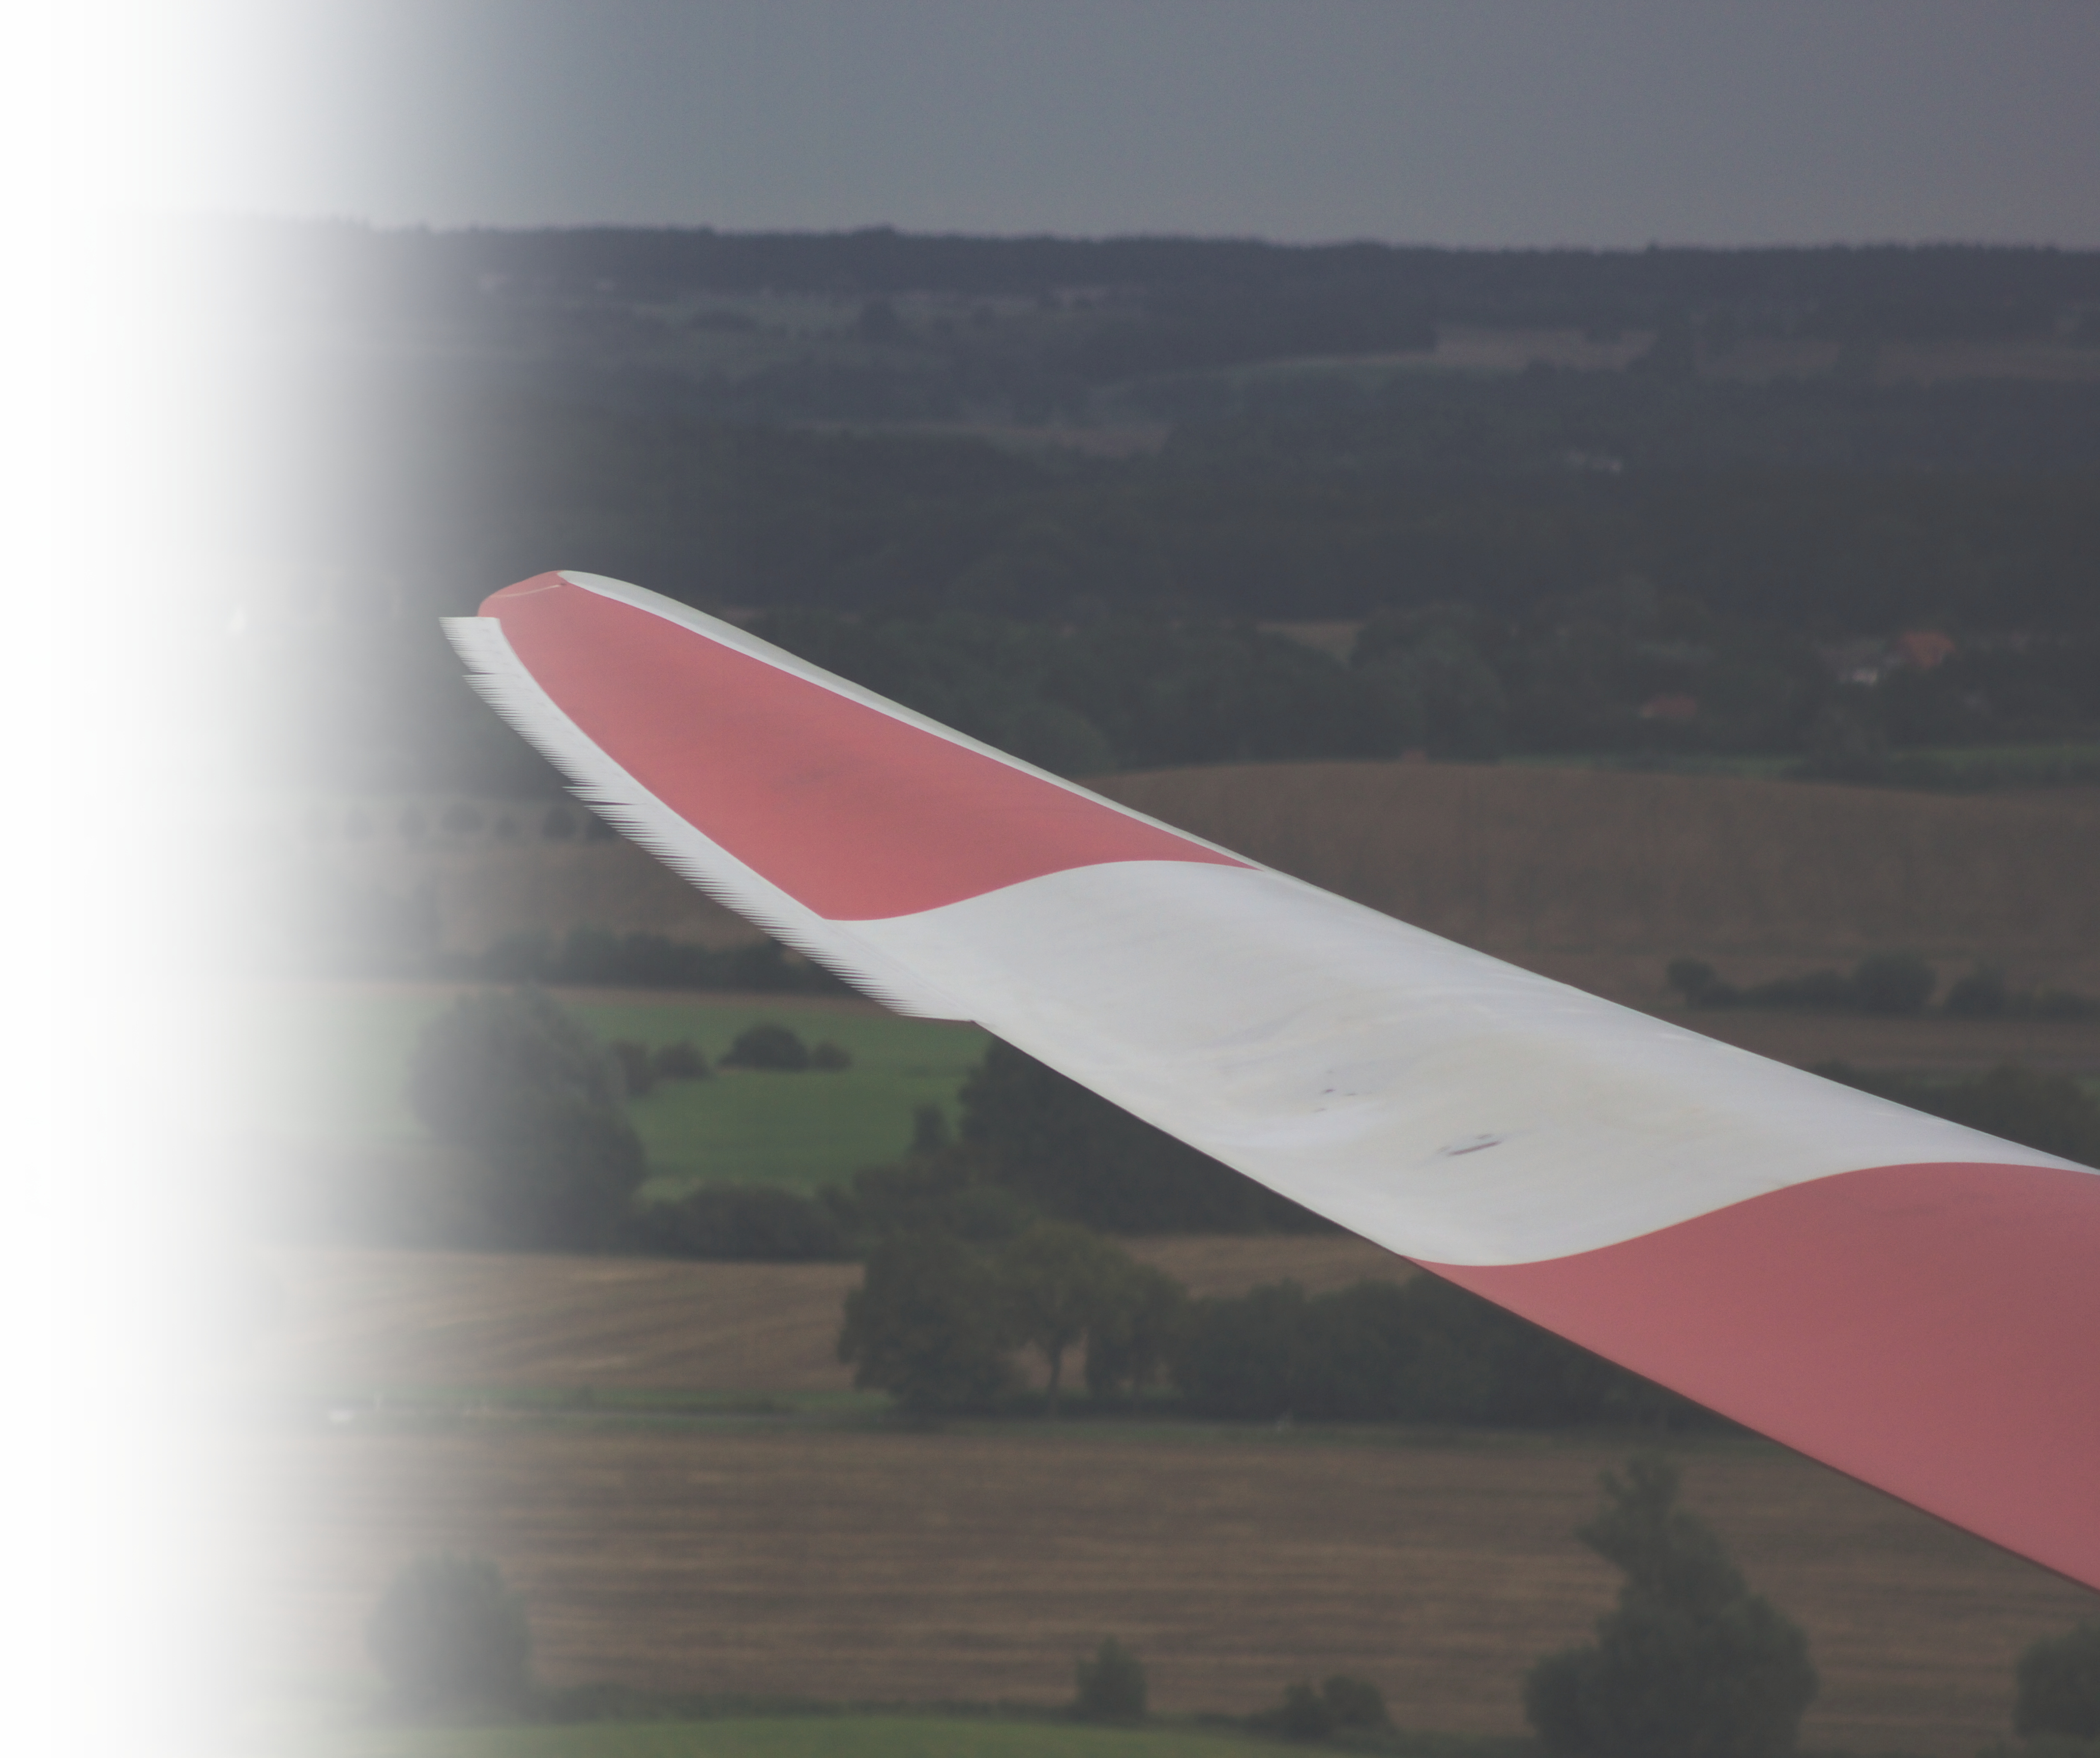
\includegraphics[height=1.1\textheight]{media/serratedBladeField.jpg}
    \end{backgroundblock}
\end{frame}

\begin{frame}[b]{The industrial application of serrations}{The need for quieter and more efficient wind turbines}
    \begin{columns}
        \column{0.5\textwidth}
        \footnotesize{Multiple challenges call for the development of reliable and robust solutions for rotor noise:
            \begin{itemize}
                \item regulations are strict and complicated\footnotemark\ in noise-sensitive regions,
                \item faster rotors help reduce drivetrain costs,
                \item there is a strong drive to enter low wind speed regions,
                \item we \emph{need} to let the people know that we care.
            \end{itemize}
        }

        \vspace{5mm}
        Ultimately, we need to keep reducing LCoE to become a more competitive source of energy.
        \vspace{5mm}
        \column{0.45\textwidth}
        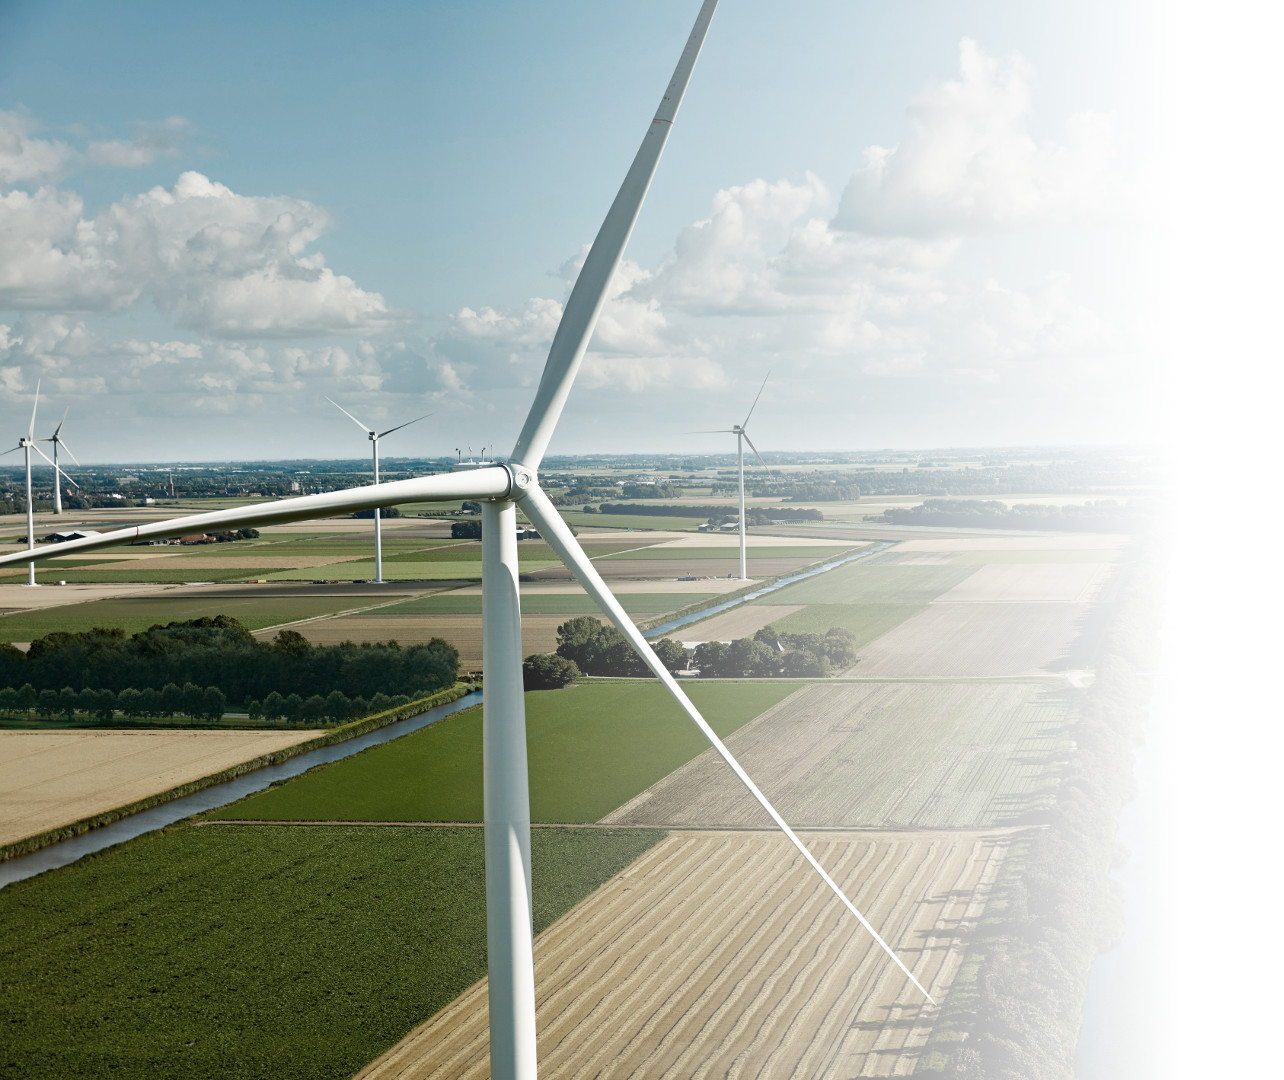
\includegraphics[width=\textwidth]{media/LM_holland_helikopter_modified.jpg}
        \vspace{6mm}
    \end{columns}
    \footnotetext{See \cite{Koppen2015}} 
\end{frame}

\begin{frame}[b]{The industrial application of serrations}{\phantom{a}}

    \begin{center}
        \vspace{1cm}
    \includemedia[
        label=wind_turbine_with_serrations,
        width=0.7\textwidth,
        activate=pagevisible,
        addresource=media/MyMovie.mp4,
        flashvars={
            source=media/MyMovie.mp4
            &autoPlay=true
            &loop=true
        }
    ]{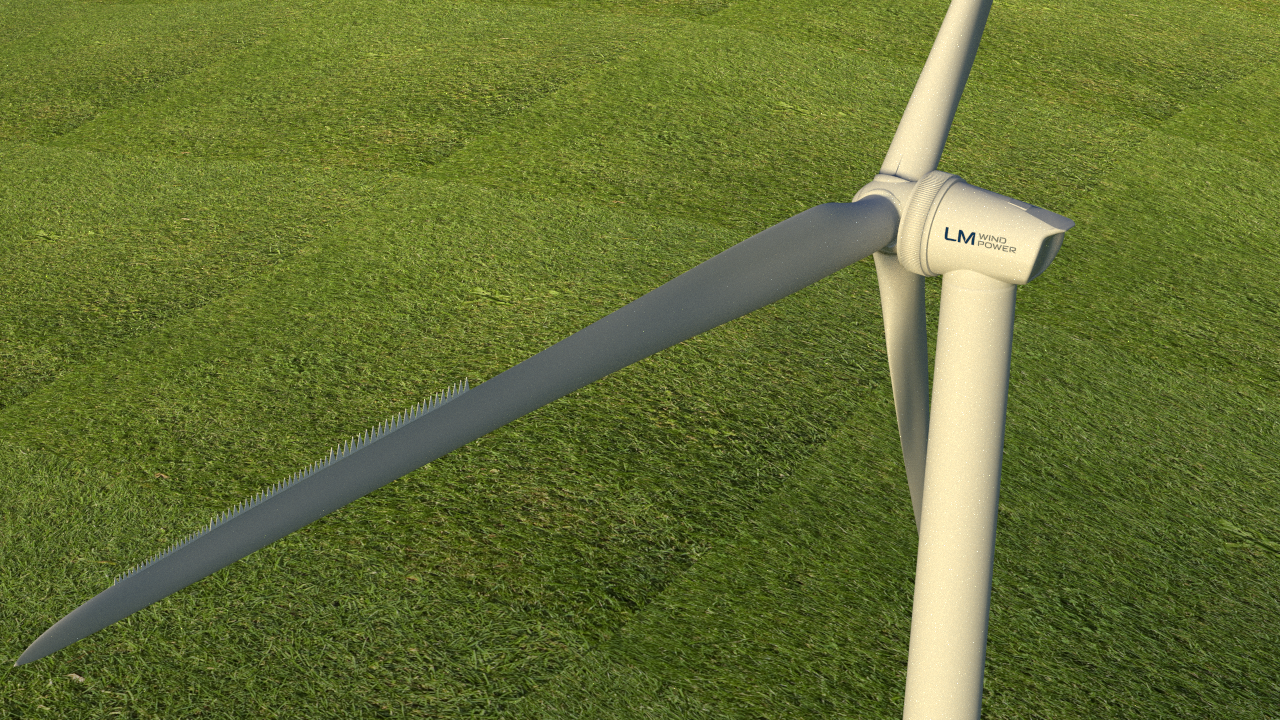
\includegraphics[width=0.5\textwidth]{media/WindTurbineWithSerrations.png}}{VPlayer.swf}
    \end{center}

    \color{LMLightBlue}{\phantom{a}
    \vspace{5mm}
 }
\end{frame}

\begin{frame}[b]{The LM serrations experience}{Creating confidence through the years}

    \centering
    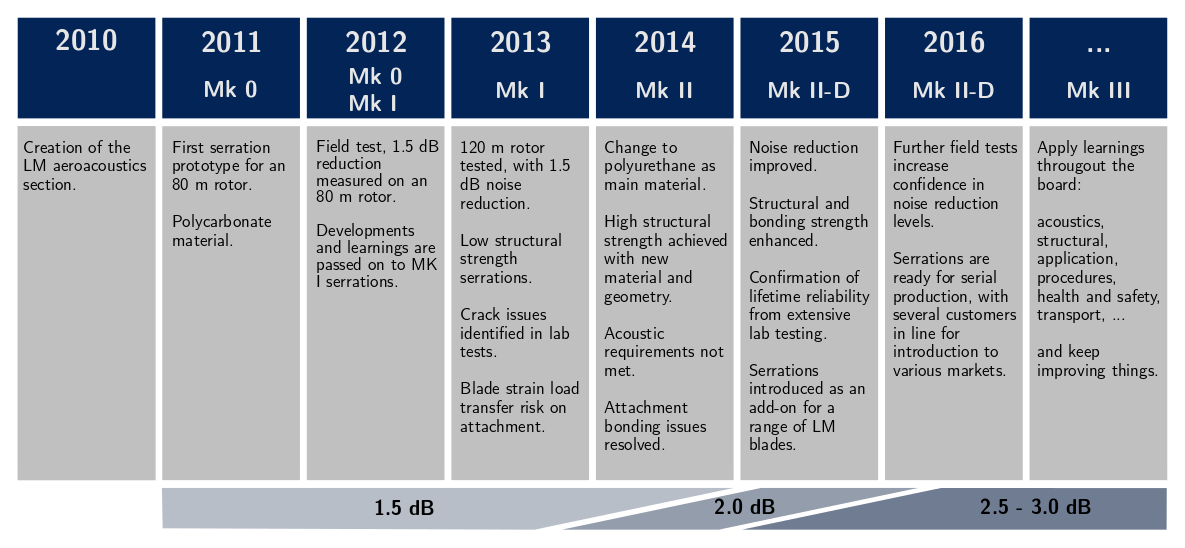
\includegraphics[width=0.95\textwidth]{media/LMSerrationHistory.png}

\end{frame}

\section{Serration-flow misalignment in other research}
\CurrentSection

\begin{frame}[b]{Flow-misaligned serrations in other research}{Some references in literature}
   \begin{columns}

      \column{0.6\textwidth}
      \scriptsize{
         \begin{quote}
             Misalignment of the teeth in this way gave rise to an \textcolor<1-2>{LMLightBlue}{increase} ($1$ to $\unit{5}{\deci\bel}$)
         \end{quote}
         \vspace{-9mm}
         \begin{flushright}
            \cite{Dassen1996}
         \end{flushright}
         \vspace{-2mm}
         \begin{quote}
             By aligning the serrations with the flow, it was attempted to minimize their aerodynamic impact and prevent \textcolor<1-2>{LMLightBlue}{increased high-frequency noise} by \alert<2>{flow through the teeth}.
         \end{quote}
         \vspace{-6mm}
         \begin{flushright}
            \cite{oerlemans2009reduction}
         \end{flushright}
         \vspace{-2mm}
         \begin{quote}
             Experimental data have shown a clear noise \textcolor<1-2>{LMLightBlue}{increase at high frequencies}, which has been interpreted to be \alert<2>{due to the cross flow through the valleys of the sawtooth structures} and the changes to the hydrodynamic field of the trailing edge
         \end{quote}
         \vspace{-6mm}
         \begin{flushright}
            \cite{Gruber2012}
         \end{flushright}
      }

      \column{0.4\textwidth}
      \vspace{0mm}
         \begin{flushright}
            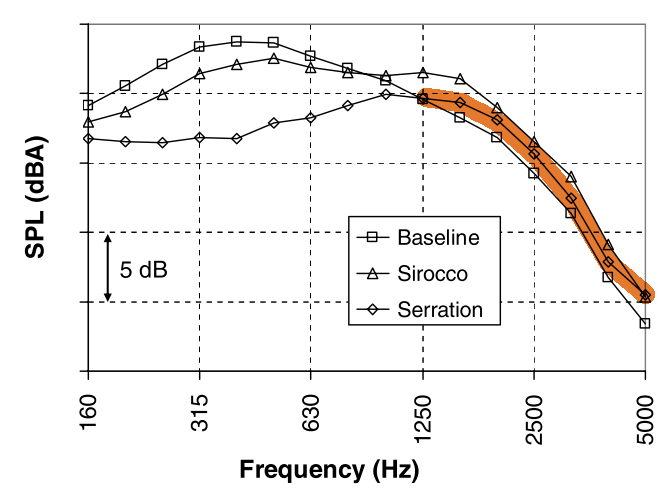
\includegraphics[width=0.6\textwidth]{./media/SerrationIncrease_oerlemans2009reduction.png}\newline
            \tiny From \cite{oerlemans2009reduction}
         \end{flushright}

         \vspace{-5mm}

         \begin{flushright}
            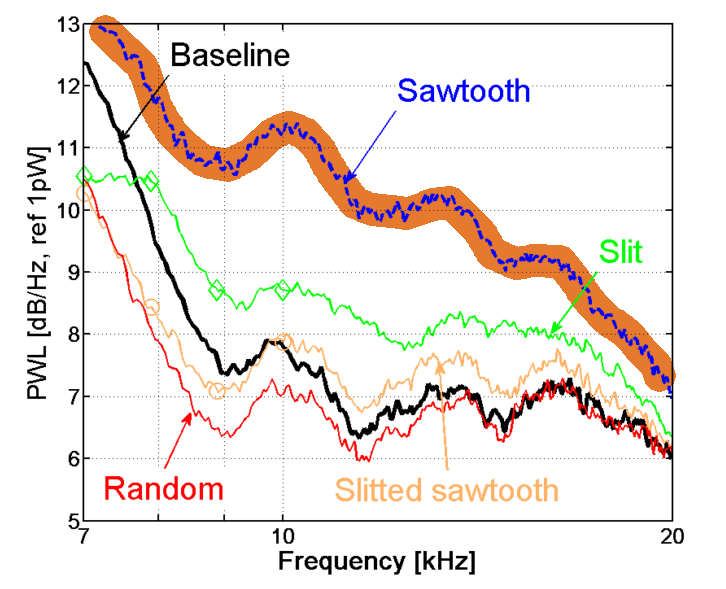
\includegraphics[width=0.6\textwidth]{./media/SerrationIncrease_Gruber2013.png}\newline
            \tiny From \cite{Gruber2013}
         \end{flushright}

   \end{columns}
   
\end{frame}

\begin{frame}[b]{Flow-misaligned serrations in other research}{Flow visualization by Gruber}
    \begin{center}
        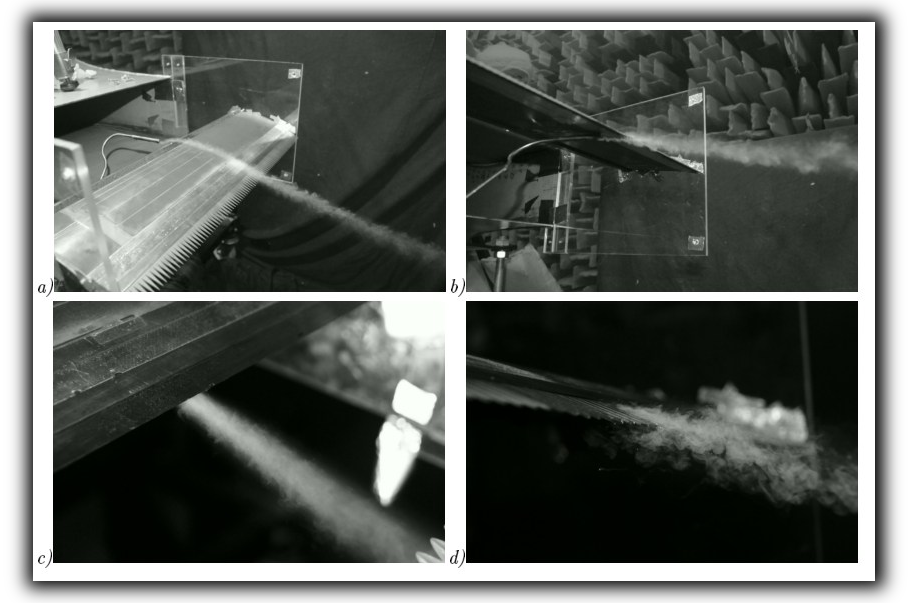
\includegraphics[width=0.55\textwidth]{media/GruberFlowViz.png}
        \begin{flushright}
            \vspace{-3mm}
            \scriptsize{
                From \cite{Gruber2011}\hspace{3cm}
            }
        \end{flushright}
    \end{center}
\end{frame}

\begin{frame}[b]{Flow-misaligned serrations in other research}{Hot-wire measurements by Gruber}
    \vspace{1cm}
    \begin{center}
        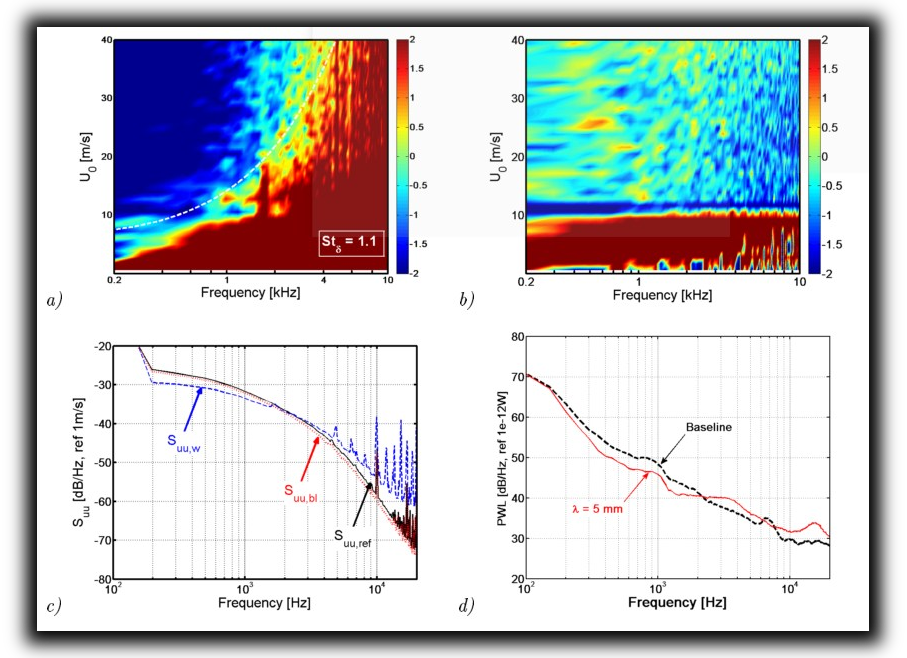
\includegraphics[width=0.60\textwidth]{media/GruberHotwireComparison.png}
        \begin{flushright}
            \vspace{-1mm}
            \scriptsize{
                From \cite{Gruber2011}\hspace{3cm}
            }
        \end{flushright}
    \end{center}
\end{frame}

\begin{frame}[b]{Flow-misaligned serrations in other research}{Gruber's Strouhal number}
    \vspace{1cm}
    \begin{center}
        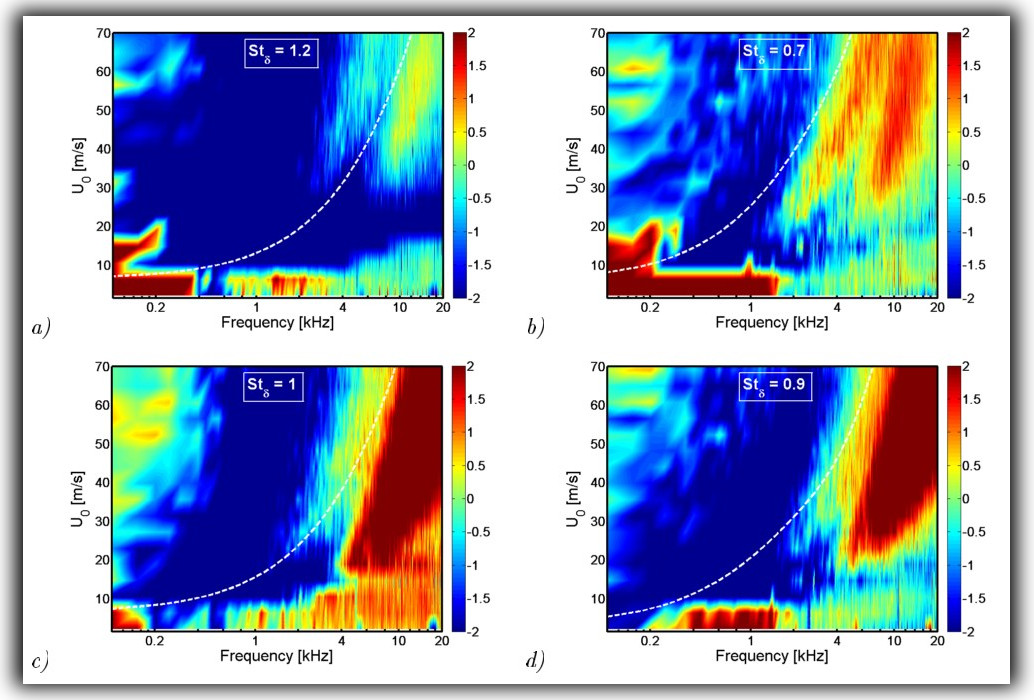
\includegraphics[width=0.60\textwidth]{media/GruberStrouhal.jpg}
        \begin{flushright}
            \vspace{-1mm}
            \scriptsize{
                From \cite{Gruber2011}\hspace{3cm}
            }
        \end{flushright}
    \end{center}
\end{frame}

\begin{frame}[c]{Flow-misaligned serrations in other research}{The investigation of \cite{Vathylakis2016}}
    \vspace{1cm}
    \begin{columns}
        \hspace{5mm}\column{0.3\textwidth}
        \begin{center}
            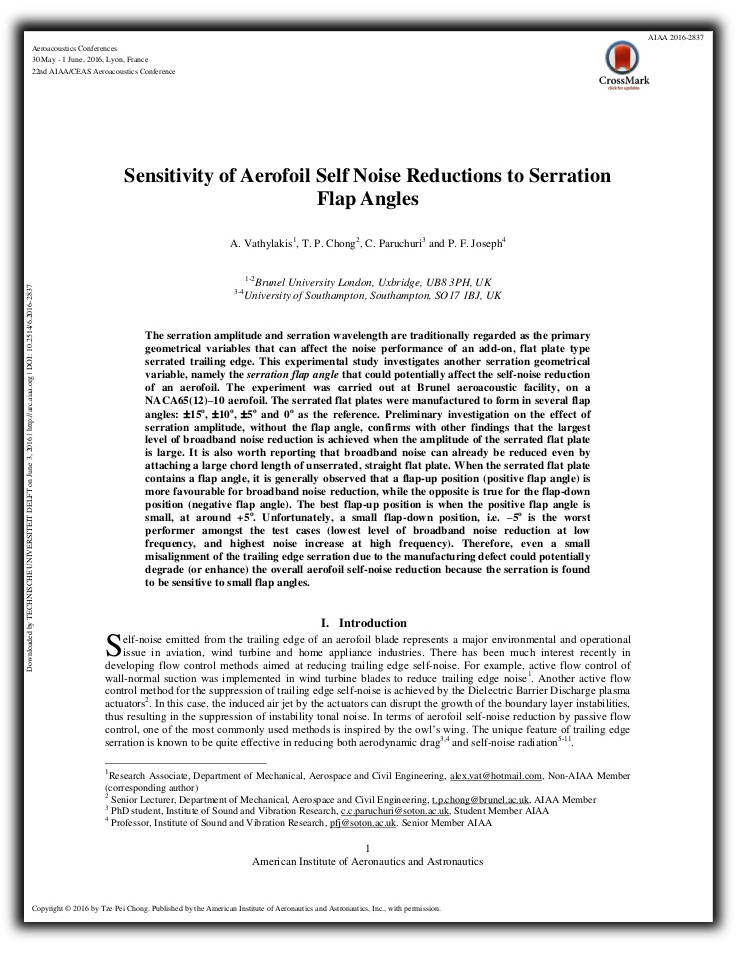
\includegraphics[width=1.00\textwidth]{media/VathylakisPage.png}
        \end{center}
        \column{0.3\textwidth}
        \begin{center}
            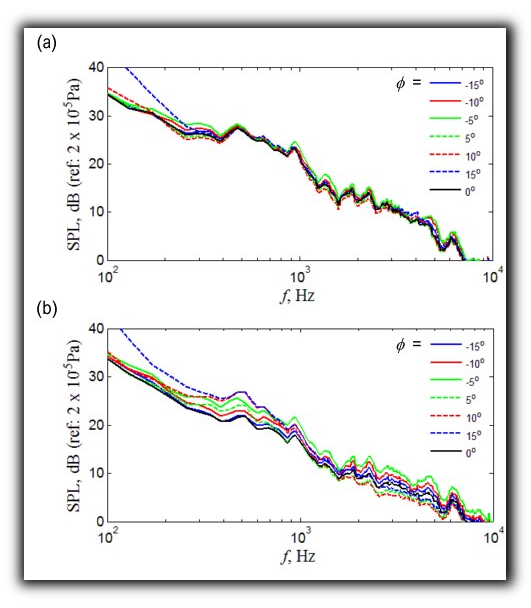
\includegraphics[width=1.00\textwidth]{media/Vathylakis1.png}
        \end{center}
        \column{0.3\textwidth}
        \begin{center}
            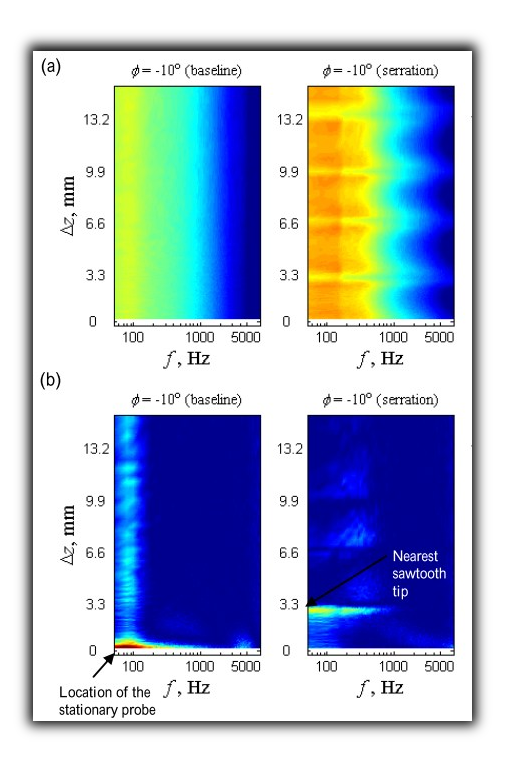
\includegraphics[width=0.90\textwidth]{media/Vathylakis2.png}
        \end{center}
    \end{columns}
\end{frame}

\begin{frame}{Plenty of work\ldots}{So what is missing?}
    \begin{itemize}
        \item A symmetric airfoil
        \item Same flow conditions on the upper and lower serration sides
        \item More near-surface and near-edge measurements
    \end{itemize}
\end{frame}

\section{Experiment setup}
\CurrentSection

\begin{frame}{}{}
    \Large \bf \textcolor{LMLightBlue}{The TU Delft \\wind tunnel campaigns}
    \begin{backgroundblock}{70mm}{0mm}
        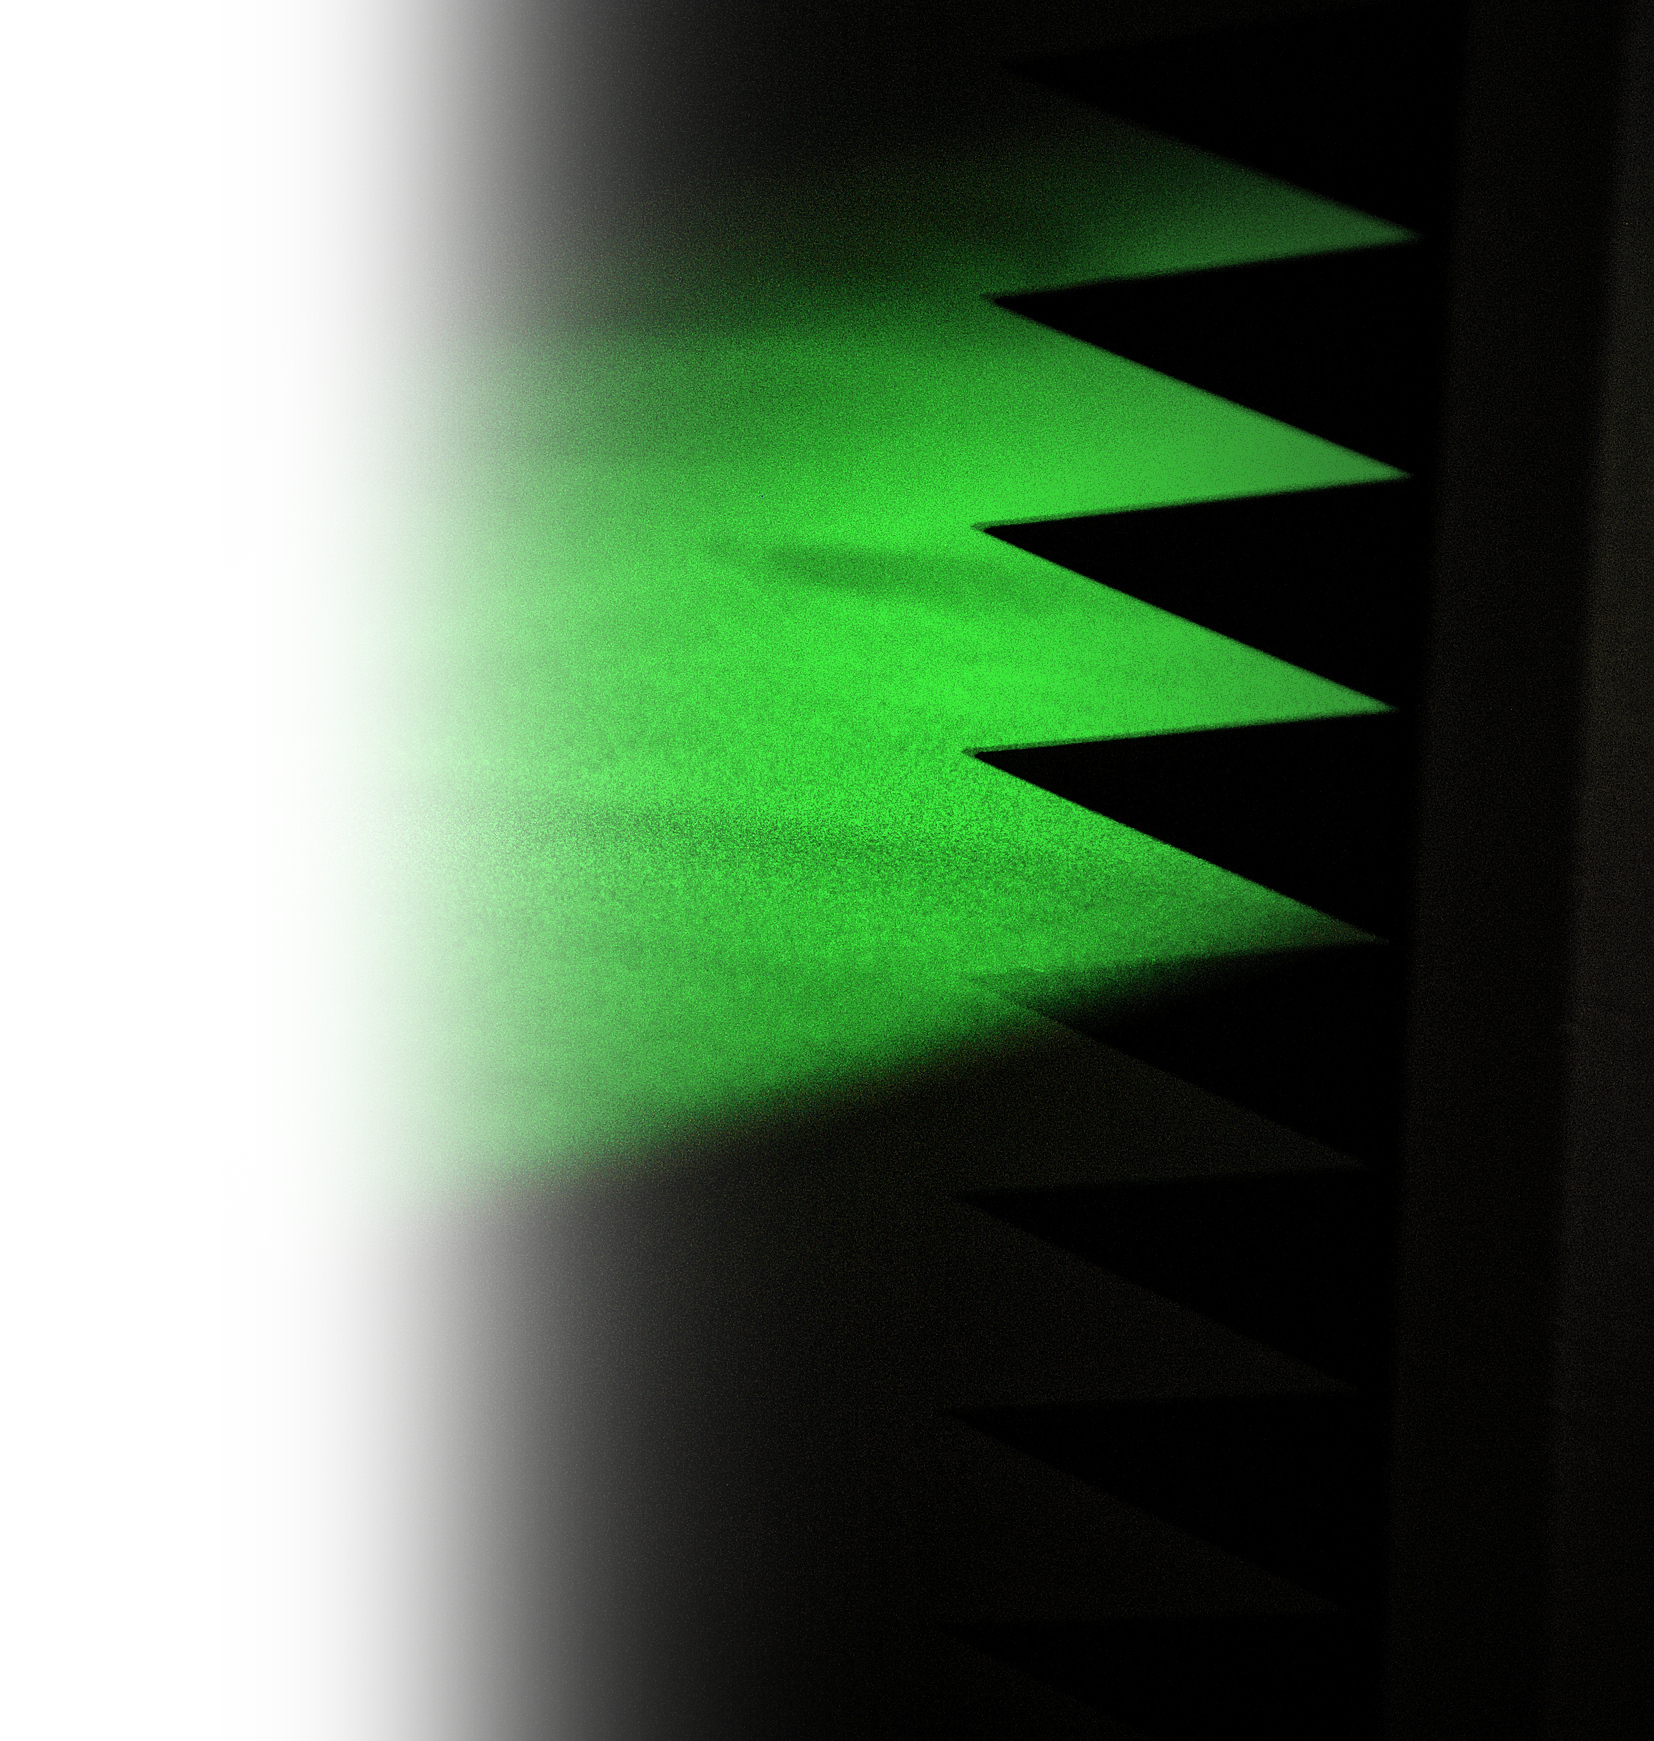
\includegraphics[height=1.1\textheight]{media/PIVSerrationBackground.jpg}
    \end{backgroundblock}
\end{frame}

\begin{frame}{The TU Delft campaigns}{Objective of the research}
    \vspace{1.0cm}
    \textcolor{LMBlue}{\bf What is the effect of this serration-flow misalignment\\on the acoustics, and---whatever it is---can it be observed \\in hydrodynamic measurements?}

    \vspace{0.5cm}

    Also\dots
    \begin{itemize}
        \item Do we also observe an \textcolor{LMLightBlue}{increase in the high-frequencies}?
        \item Does the \textcolor{LMLightBlue}{Strouhal $\sim 1$} relation hold in our case?
        \item If it does, \textcolor{LMLightBlue}{does it change} with $\alpha$ and $\varphi$?
        \item Can we \textcolor{LMLightBlue}{localize the source} of this noise increase?
    \end{itemize}
\end{frame}

\begin{frame}{The TU Delft campaigns}{Acknowledgements}
    \vspace{0.5cm}\hspace{1cm}
    \begin{tabular}{ll}
        D. Ragni             & T\textcolor{LMLightBlue}{U} Delft, Aeroacoustics \\
        F. Avallone          & T\textcolor{LMLightBlue}{U} Delft, Aeroacoustics \\
        S. Pr\"obsting       & T\textcolor{LMLightBlue}{U} Delft, Aerodynamics \\
        R. Merino-Mart\'inez & T\textcolor{LMLightBlue}{U} Delft, ANCE\\
    \end{tabular}
\end{frame}

\begin{frame}{Experiment setup}{\alert{Wind tunnel} + airfoil \& serrations + PIV + acoustics}

    \textcolor{LMBlue}{\bf Facility}
    \begin{itemize}
        \item TU Delft V-Tunnel,
        \item $\unit{20}{\metre\per\second}$ (PIV), 30, 35 and $\unit{40}{\metre\per\second}$ (acoustics),
        \item $\unit{20}{\metre\per\second}\approx\unit{263\,000}{Re}$,
        \item nozzle of $40\times\unit{40}{\centi\metre\squared}$,
        \item large contraction, low turbulence at exit $\left( <1\% \right)$.
    \end{itemize}
    
\end{frame}

\begin{frame}{Experiment setup}{Wind tunnel + \alert{airfoil \& serrations} + PIV + acoustics}

    \begin{columns}
        \column{0.5\textwidth}
        \vspace{1cm}
        \def\svgwidth{1.0\textwidth} 
        {\scriptsize \input{AirfoilDimensions.pdf_tex}}

        \column{0.5\textwidth}
        \begin{itemize}
            \item NACA 0018,
            \item forced transition with trip at $0.2\,C$,
            \item $\alpha^* = \unit{0}{\degree},\,\unit{3.3}{\degree},\,\unit{6.6}{\degree}$,
            \item $\varphi = \unit{0}{\degree},\,\unit{6}{\degree}$.
        \end{itemize}

    \end{columns}
    
\end{frame}

\begin{frame}{Experiment setup}{Wind tunnel + airfoil \& serrations + \alert{PIV} + acoustics}

    \begin{columns}
        \column{0.45\textwidth}
        \vspace{1cm}
        \begin{itemize}
            \item High-speed ($\unit{10}{\kilo\hertz}$)
            \item Stereoscopic
        \end{itemize}
        \vspace{5mm}
        \centering
        \def\svgwidth{0.5\textwidth} 
        {\scriptsize \input{FieldOfView3D.pdf_tex}}

        \column{0.55\textwidth}
        \includemedia[
            label=sPIVsetup,
            width=0.9\textwidth,
            height=0.50625\textwidth,
            activate=pagevisible,
            addresource=media/WallNormalPlanesSetup.mp4,
            flashvars={
                source=media/WallNormalPlanesSetup.mp4
                &autoPlay=true
            }
        ]{\vspace{3.0cm}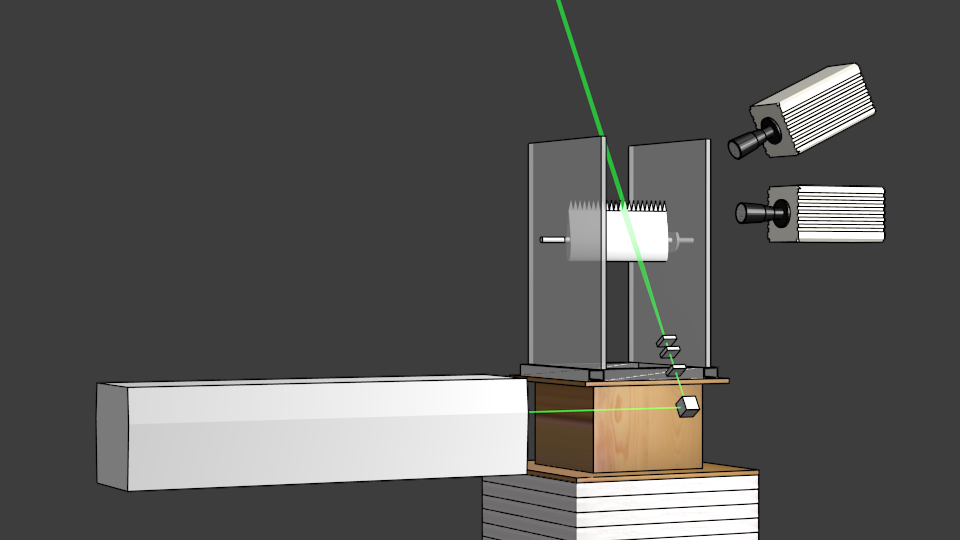
\includegraphics[width=0.5\textwidth]{media/WallNormalPlanesSetup.png}}{VPlayer.swf}
    \end{columns}
    
\end{frame}

\begin{frame}{Experiment setup}{Wind tunnel + airfoil \& serrations + PIV + \alert{acoustics}}

    \begin{columns}
        \column{0.5\textwidth}
        \vspace{-1.5cm}
        \centering
                \includemedia[
                    label=Acousticsetup,
                    height=0.7\textwidth,
                    activate=pagevisible,
                    addresource=media/AnechoicTunnelSetup.mp4,
                    flashvars={
                        source=media/AnechoicTunnelSetup.mp4
                        &autoPlay=true
                    }
                ]{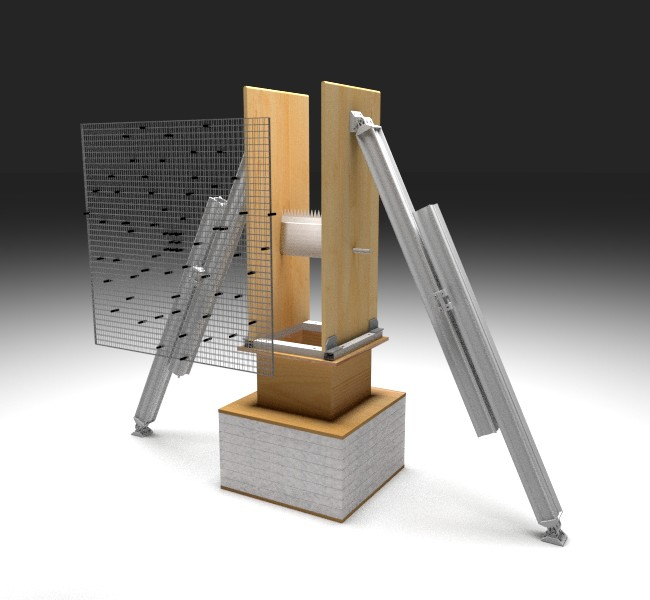
\includegraphics[width=0.3\textwidth]{media/AnechoicTunnelSetup.jpg}}{VPlayer.swf}
    
        \column{0.5\textwidth}
        \vspace{1cm}
        \begin{itemize}
            \item 64-mic array
            \item $\unit{0.9}{\metre}$ effective diameter
            \item 1 to $\unit{5}{\kilo\hertz}$ frequency range
            \item $\unit{60}{\second}$ measurements at $\unit{50}{\kilo\hertz}$ sampling frequency
            \item 2048 block length with Hanning windowing and 50\% overlap
        \end{itemize}

    \end{columns}

\end{frame}

\section{Results}
\CurrentSection

\begin{frame}{Acoustic results}{So do serrations reduce noise? (of course they do)}

    \begin{columns}
        \column{0.5\textwidth}
        \vspace{-2cm}
        \centering
        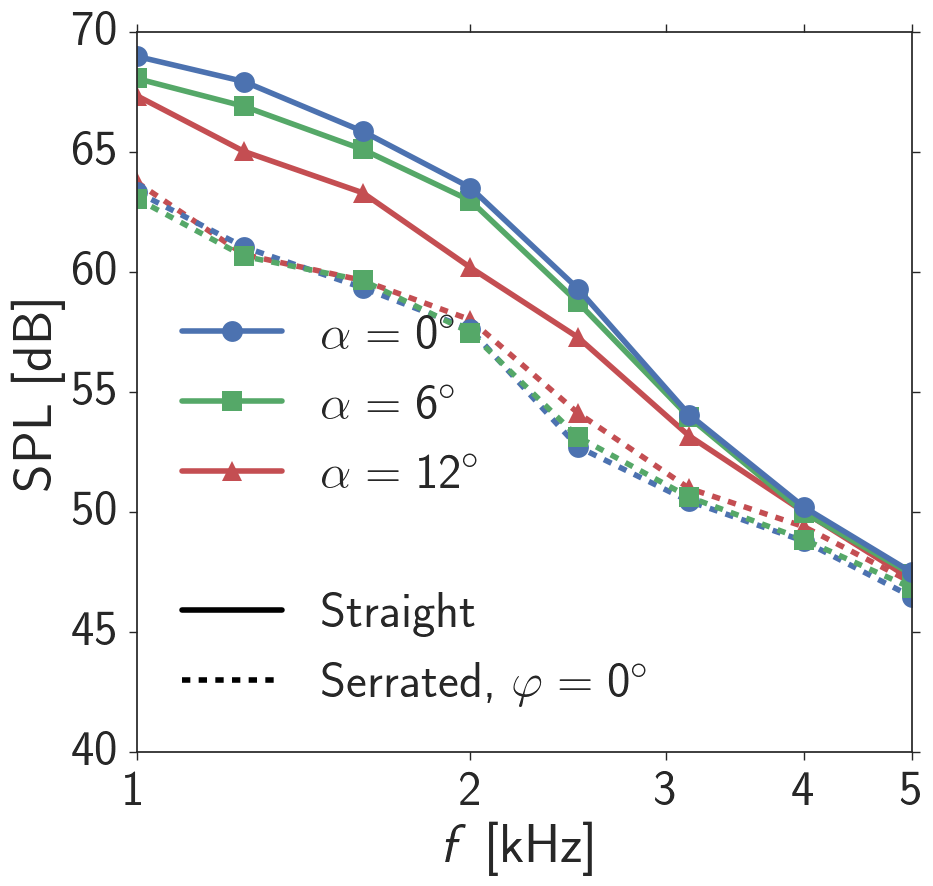
\includegraphics[width=0.8\textwidth]{scripts/acoustics/article_images/case35_spectra_p0.png}
        \column{0.5\textwidth}
    \end{columns}
    
\end{frame}

\begin{frame}{Acoustic results}{Evidence of the high-frequency noise increase}

    \begin{columns}
        \column{0.5\textwidth}
        \vspace{-2cm}
        \centering
        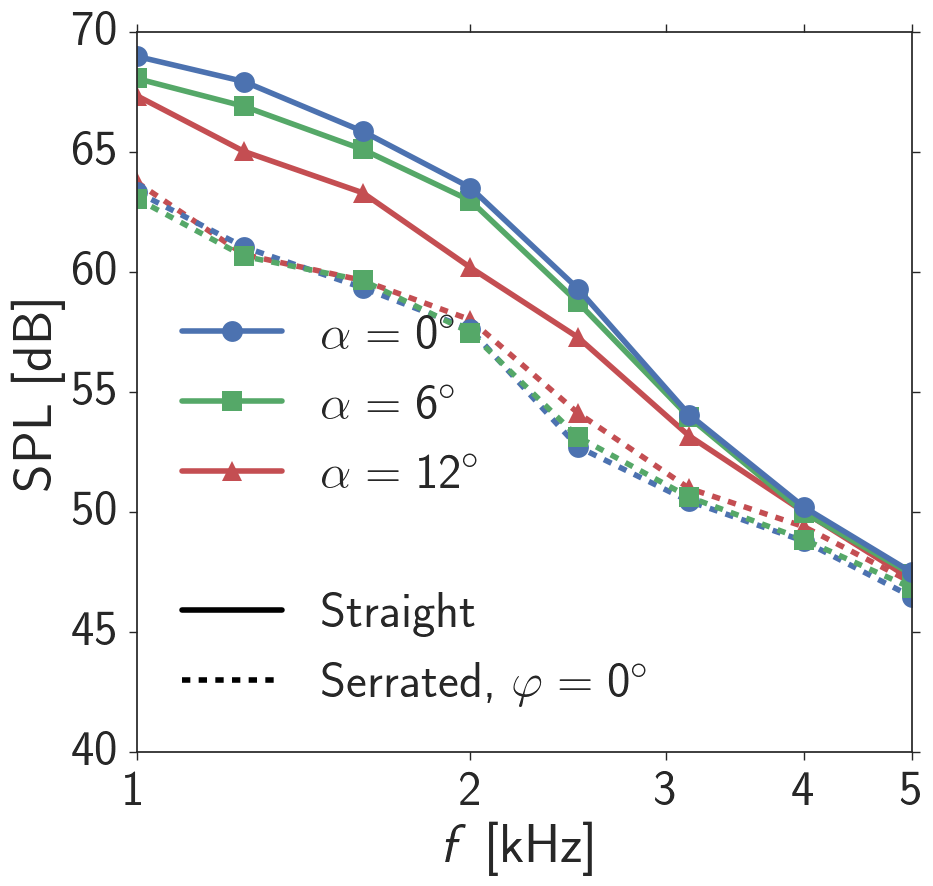
\includegraphics[width=0.8\textwidth]{scripts/acoustics/article_images/case35_spectra_p0.png}
        \column{0.5\textwidth}
        \vspace{-2cm}
        \centering
        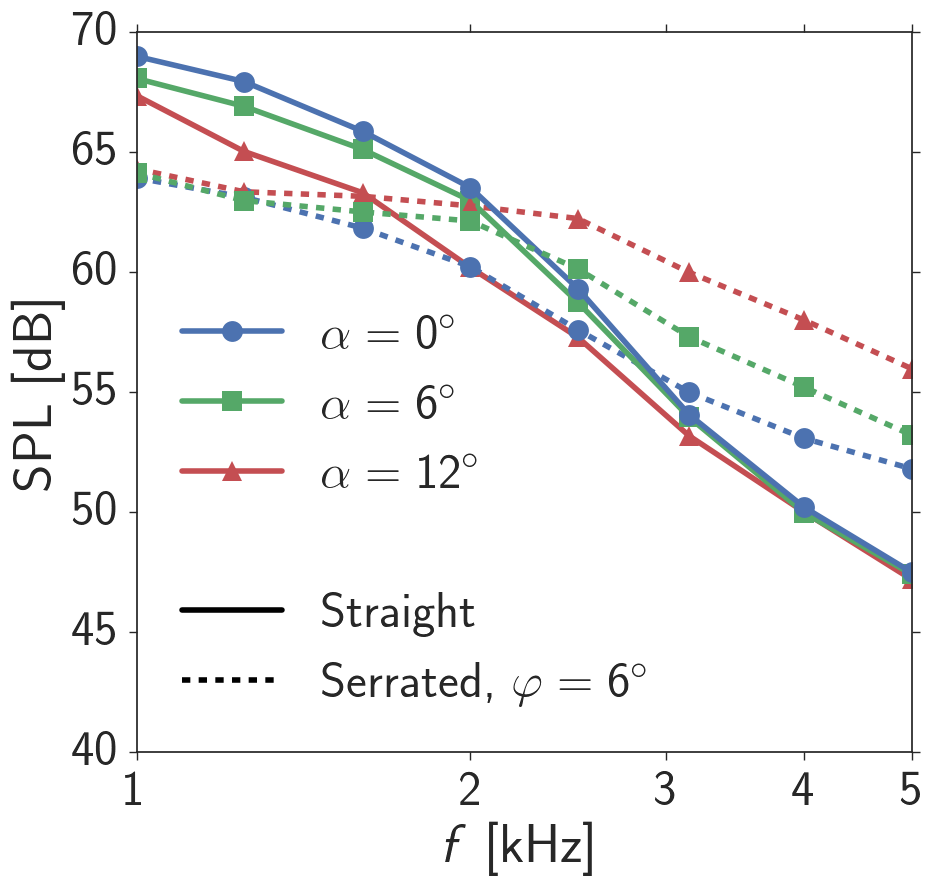
\includegraphics[width=0.8\textwidth]{scripts/acoustics/article_images/case35_spectra_p6.png}
    \end{columns}
    
\end{frame}

\begin{frame}{Acoustic results}{Source map comparison}

    \vspace{1cm}
    \centering
    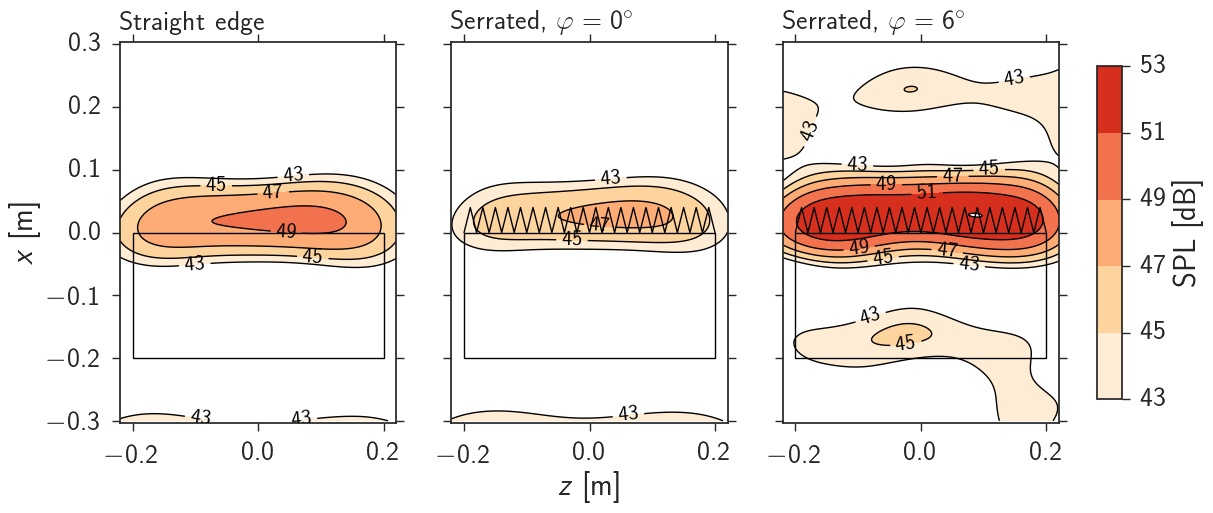
\includegraphics[width=0.8\textwidth]{scripts/acoustics/results/SourceMap.png}
    
\end{frame}

\begin{frame}{Acoustic results}{Evidence of the high-frequency noise increase}

    \vspace{2cm}
    \begin{columns}
        \column{0.3\textwidth}
        \centering
        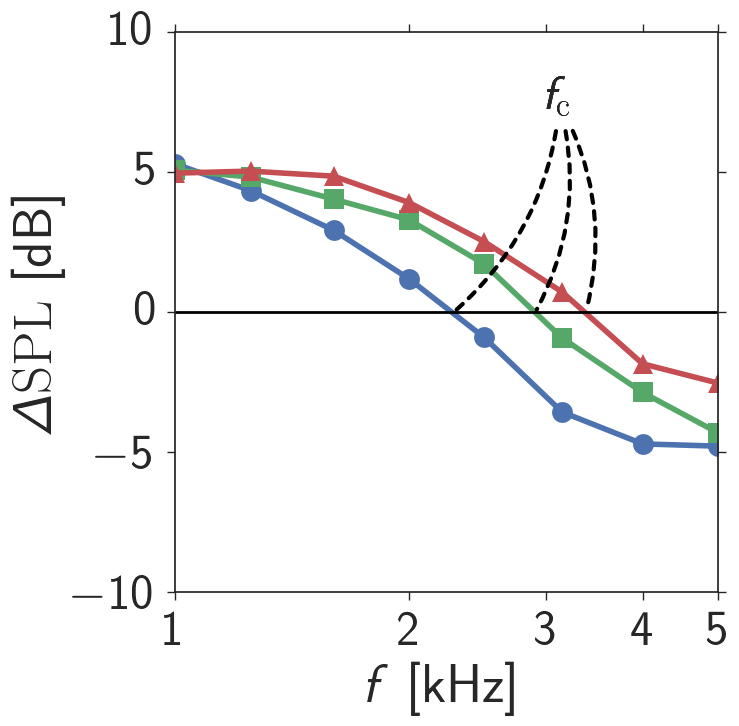
\includegraphics[width=0.8\textwidth]{scripts/acoustics/article_images/Relative_a0_p6.png}
        \column{0.3\textwidth}
        \centering
        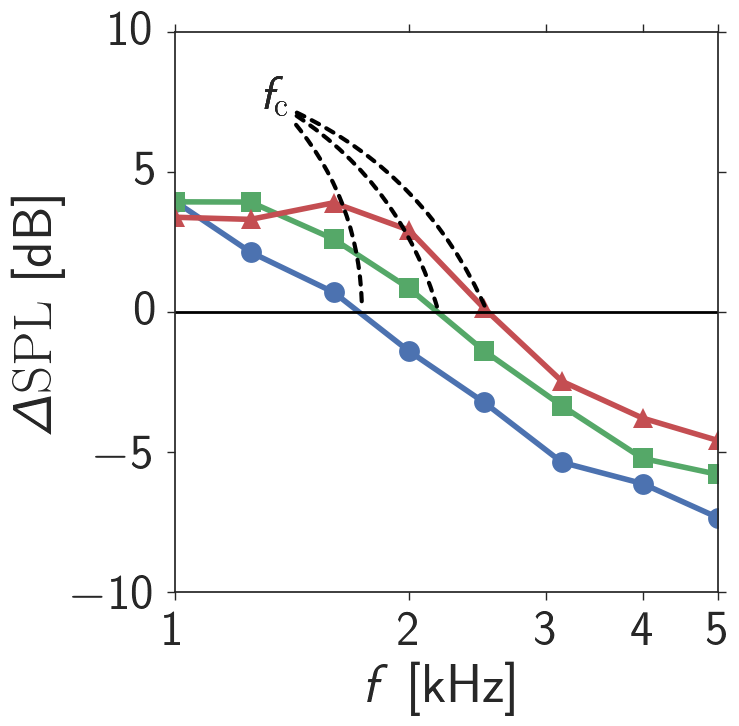
\includegraphics[width=0.8\textwidth]{scripts/acoustics/article_images/Relative_a6_p6.png}
        \column{0.4\textwidth}
        \centering
        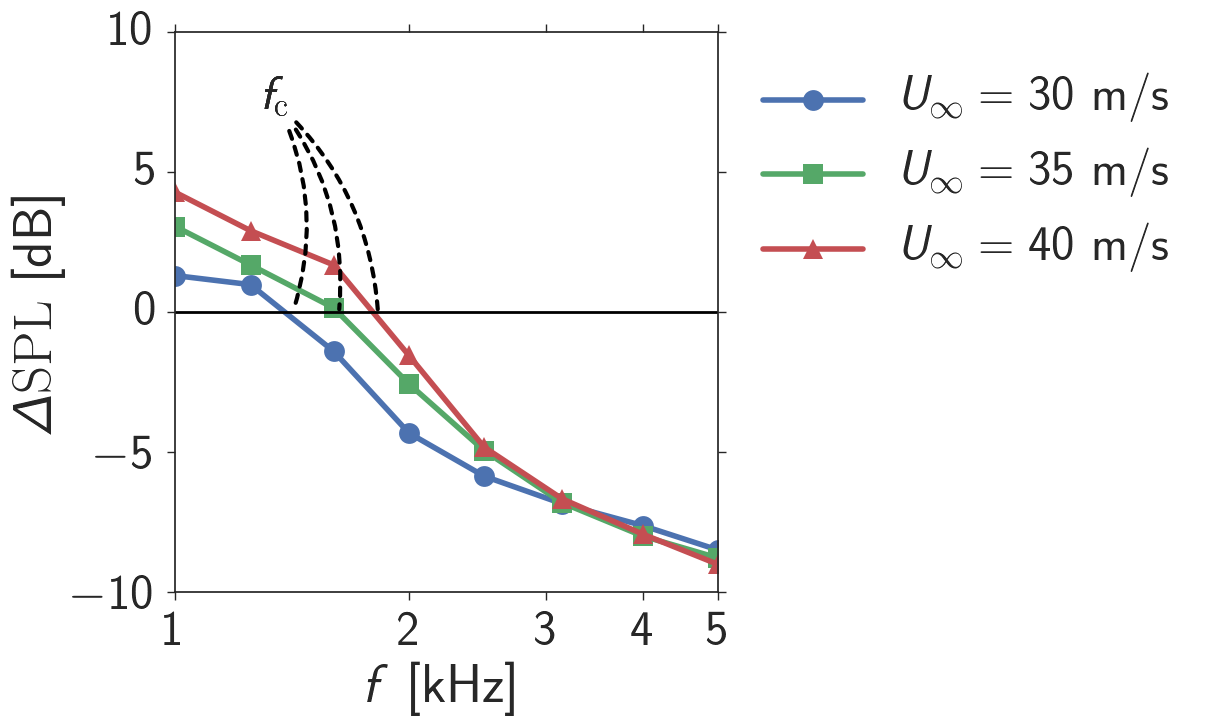
\includegraphics[width=0.95\textwidth]{scripts/acoustics/article_images/Relative_a12_p6.png}
    \end{columns}

    \begin{flushright}
        \scriptsize{$f_c$: crossover frequency}
    \end{flushright}
    
\end{frame}

\begin{frame}[b]{Acoustic results}{So, does $\mathrm{St_c}\sim 1$ hold?}

    \begin{columns}
        \column{0.55\textwidth}
        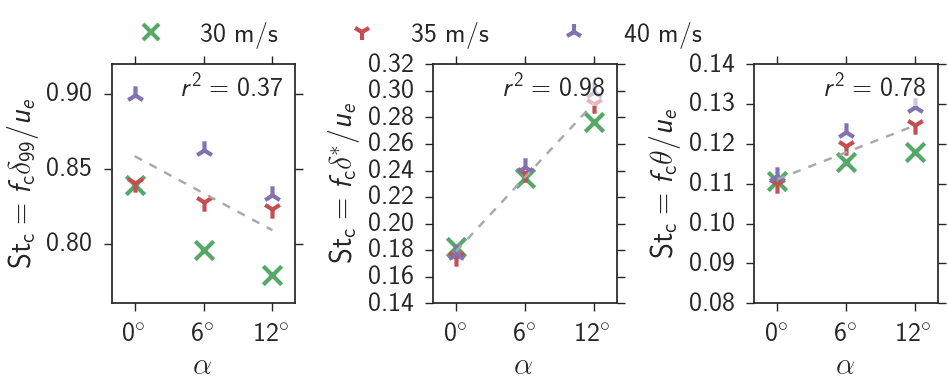
\includegraphics[width=1.\textwidth]{./scripts/acoustics/article_images/Crossover_Strouhal_and_AoA_SS.png}\\
        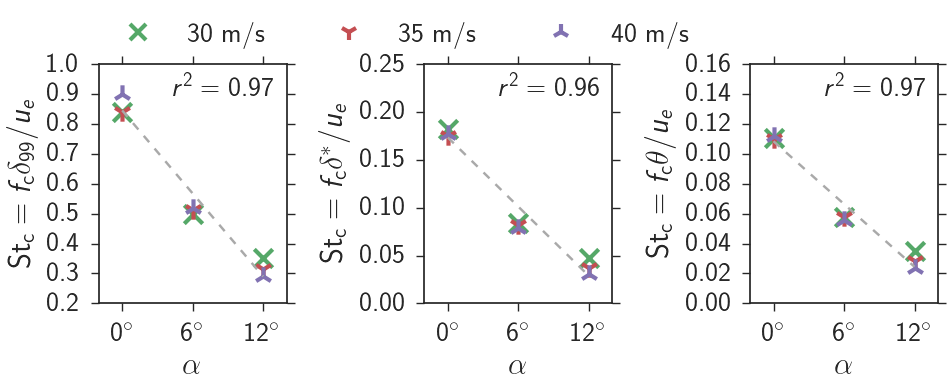
\includegraphics[width=1.\textwidth]{./scripts/acoustics/article_images/Crossover_Strouhal_and_AoA_PS.png}
        \column{0.45\textwidth}
        \only<2->{\scriptsize{
        Nope\dots but it's constancy is not totally off:
        \begin{itemize}
            \item it's ok for varying $U_\infty$ (so Gruber is right),
            \item (but not for all boundary layer measures),
            \item so when in doubt, bet on $\delta^*_\mathrm{PS}$.
            \item $\mathrm{St}$ changes linearly for $\alpha$, 
            \item and we can only guess it also depends on $\varphi$
        \end{itemize}
    }}

    \vspace{1cm}
    \only<2>{\phantom{\scriptsize{
        This is going to help us later\ldots
    }}}
    \only<3>{\scriptsize{
        This is going to help us later\ldots
    }}
    \end{columns}
    
\end{frame}

\begin{frame}{Hydrodynamics}{On to the flow\ldots}
    \bf \textcolor{LMBlue}{So what does serration-flow misalignment do\\to the mean flow?}
\end{frame}

\begin{frame}[b]{Hydrodynamics}{Near-surface mean flow (suction side)}
    \begin{center}
    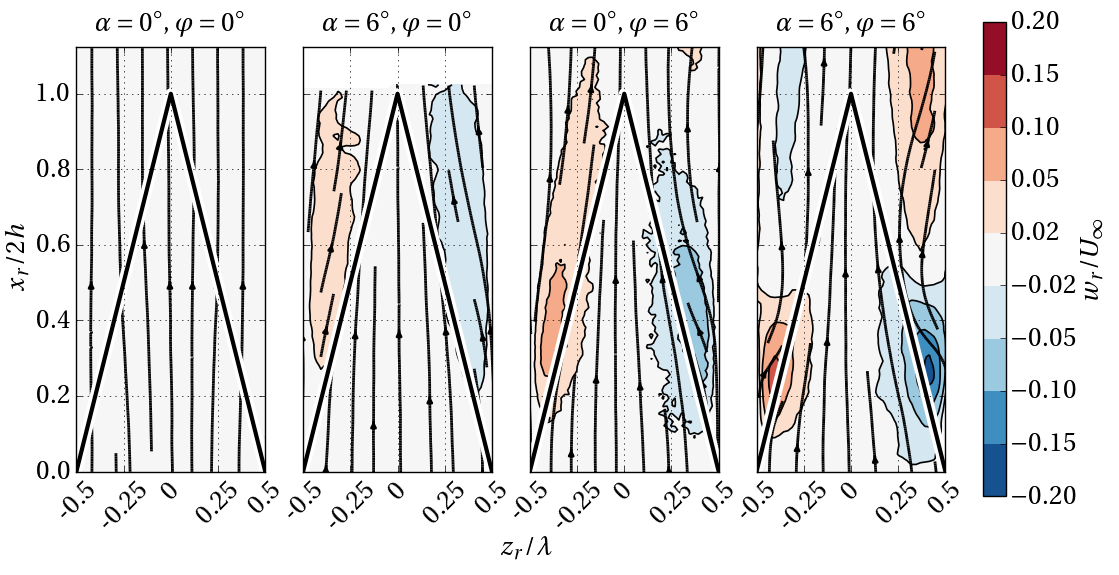
\includegraphics[width=0.8\textwidth]{./media/NearSurface-PIV_SidewaysFlowComparisonSS.png}\\
    \end{center}
\end{frame}

\begin{frame}[b]{Hydrodynamics}{Near-surface mean flow (pressure side)}
    \begin{center}
    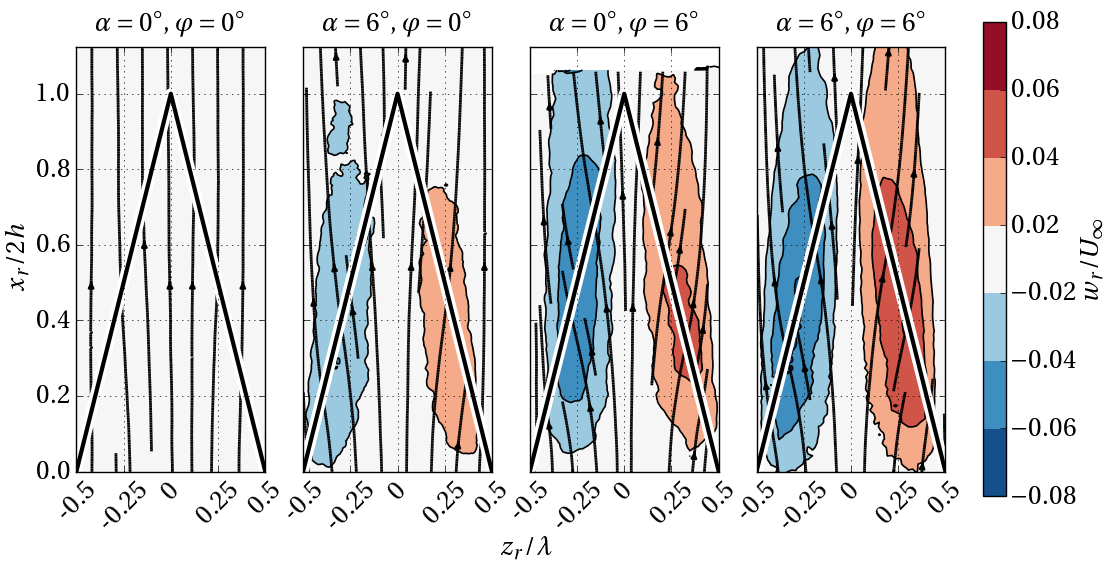
\includegraphics[width=0.8\textwidth]{./media/NearSurface-PIV_SidewaysFlowComparisonPS.png}
    \end{center}
\end{frame}

\begin{frame}[b]{Hydrodynamics}{Wake flow (vorticity)}
    \vspace{1cm}
    \begin{center}
    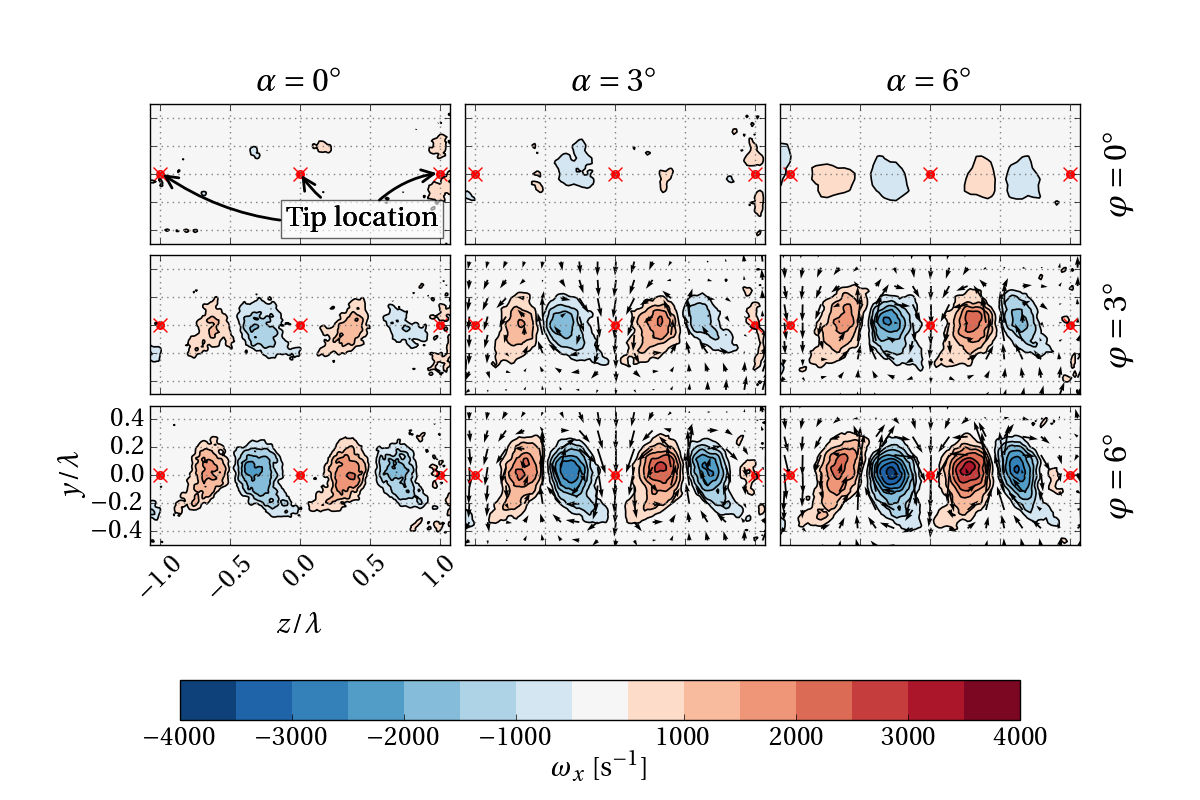
\includegraphics[width=0.70\textwidth]{./media/VorticityMatrix.png}
    \end{center}
\end{frame}

\begin{frame}{Hydrodynamics}{A bit more 3D\ldots with tomographic PIV}
    \vspace{1cm}
    \begin{center}
            \includemedia[
                label=wind_turbine_with_serrations,
                width=0.5\textwidth,
                activate=pagevisible,
                addresource=media/TomoSolidResults.mp4,
                flashvars={
                    source=media/TomoSolidResults.mp4
                    &autoPlay=true
                } ]{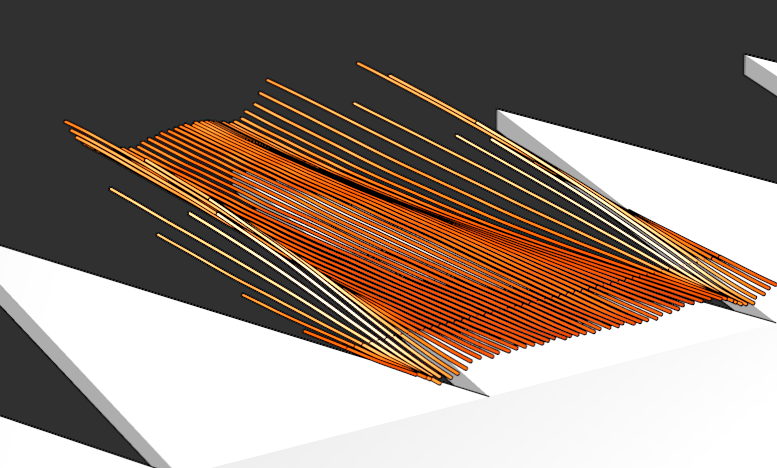
\includegraphics[width=0.5\textwidth]{media/TomoSolidResults.png}}{VPlayer.swf} 
    \end{center}
\end{frame}

\begin{frame}[b]{Boundary layer characterization}{Streamwise mean flow and rms}
    \begin{columns}
        \column{0.4\textwidth}
        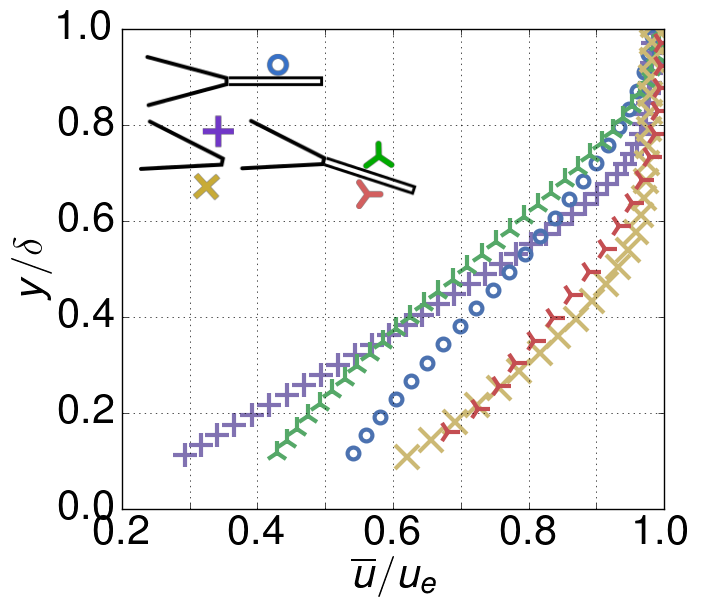
\includegraphics[width=1.0\textwidth]{./scripts/flow/time_resolved/Results/Um.png}
        \column{0.6\textwidth}
        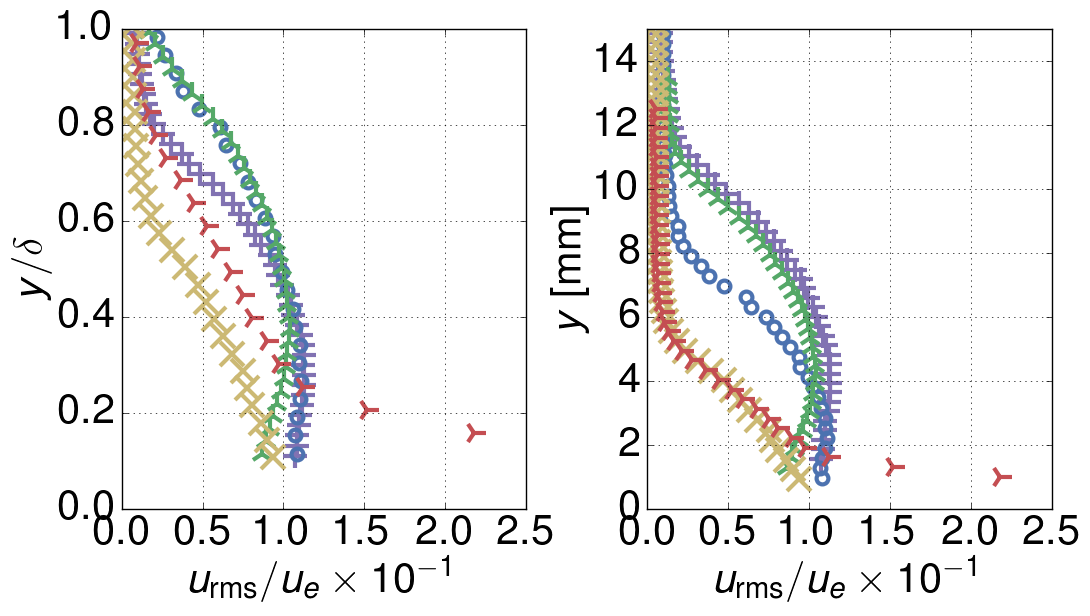
\includegraphics[width=1.0\textwidth]{./scripts/flow/time_resolved/Results/urms.png}
    \end{columns}
    \vspace{1cm}
\end{frame}

\begin{frame}[b]{Boundary layer characterization}{Streamwise length scales}
    \begin{center}
    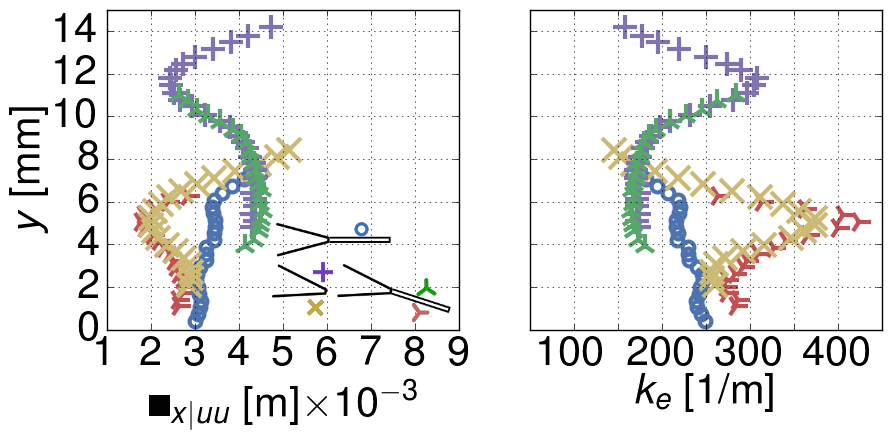
\includegraphics[width=0.5\textwidth]{./scripts/flow/time_resolved/Results/StreamwiseLengthScales_real_yloc.png}
    \end{center}
    \begin{center}
        \scriptsize{
            $\Lambda_{x|uu} \approx {\displaystyle \int_{0\,\left( \delta_\mathrm{min} \right)}^{\delta}\frac{\overline{u\left( x \right) \cdot u\left( x+\xi \right)}}{u^2\left( x \right)}}$\hspace{1cm}$k_e \approx {\displaystyle \frac{\sqrt{\pi}}{\Lambda_{x|uu}}\frac{\Gamma\left( 5/6 \right)}{\Gamma\left( 1/3 \right)}}$
        }
    \end{center}
    \vspace{0.5cm}
\end{frame}

\begin{frame}[t]{Boundary layer characterization}{Turbulence spectra}
    \vspace{1cm}
    \begin{columns}
        \column{0.6\textwidth}
        \begin{center}
            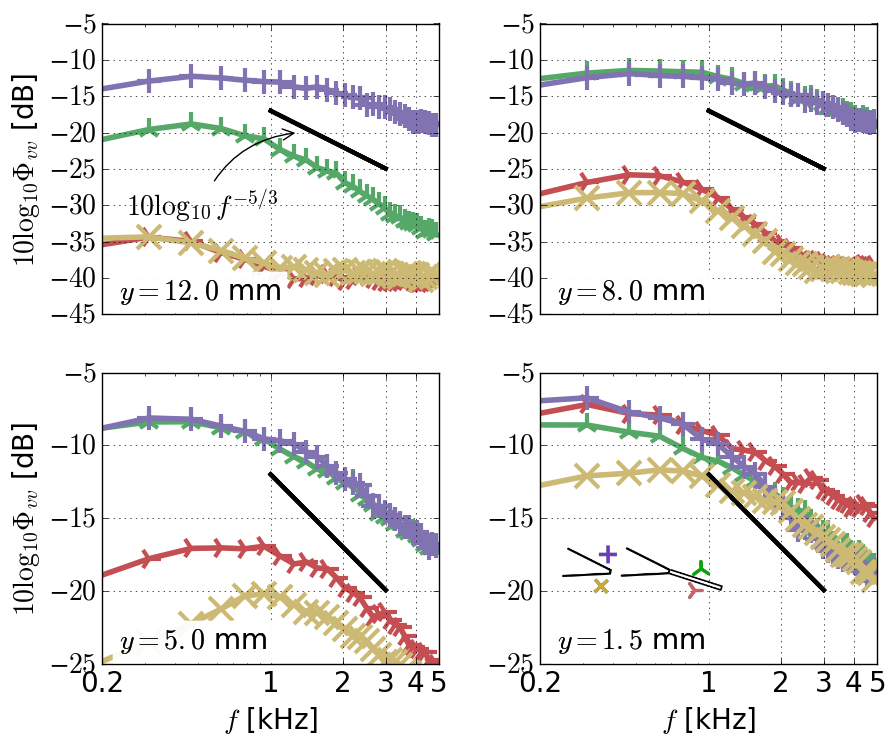
\includegraphics[width=0.8\textwidth]{./scripts/flow/time_resolved/Results/f_plot.png}
            \vspace{1cm}
        \end{center}
        \column{0.4\textwidth}
        \only<2->{
            \scriptsize{
                So does this \emph{flow} crossover near the PS edge correlate to the \emph{acoustic} crossover?
                \begin{equation*}
                    \mathrm{St}\left( U_\infty,\only<3>\alert{f_{c,\mathrm{acoustic}}},\delta^* \right) = \frac{\delta^*\only<3>\alert{f_{c,\mathrm{acoustic}}} }{U_{\infty}}
                \end{equation*}
                \only<1-3>{\textcolor{white}}{which for this case gives
                    \begin{equation*}
                        f_{c,\mathrm{acoustic}}\approx\only<4>\alert{\unit{1.1}{\kilo\hertz}}
                    \end{equation*}
                    and is around where $f_{c,\mathrm{flow}}$ is.
                }
            }
        }
    \end{columns}
\end{frame}

\begin{frame}{Take-away observations}
    \begin{columns}
        \column{0.7\textwidth}
    \begin{itemize}
        \item The noise is \alert{not from a quadrupole source} (not the volume between the teeth)
        \item It comes rather from \alert{increased energy of small eddies} near the pressure side surface edge
        \item It is still amazing \alert{how well serrations work} despite the large flow disruption
    \end{itemize}
    \column{0.3\textwidth}
    \end{columns}
\end{frame}

\begin{frame}{So, can we avoid those effects?}{Maybe serrations should not \emph{just} be triangles}
    \begin{columns}
        \column{0.3\textwidth}
        \begin{itemize}
            \item solutions with slits
            \item flexible serrations
            \item \ldots
            \item oh, so many other options
        \end{itemize}
        \column{0.3\textwidth}
        \only<2->{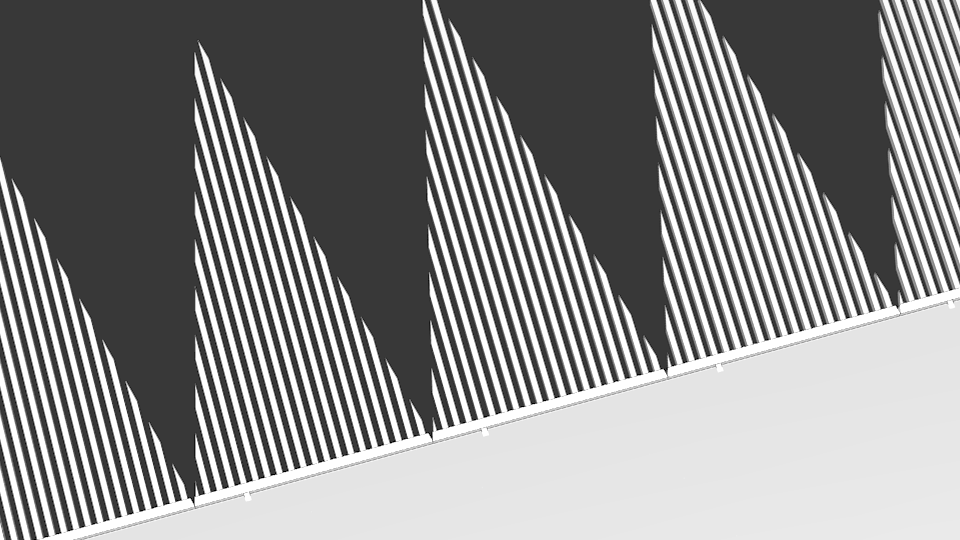
\includegraphics[width=0.9\textwidth]{media/SlittedSerrationsPoster.png}}
        \column{0.3\textwidth}
        \only<3->{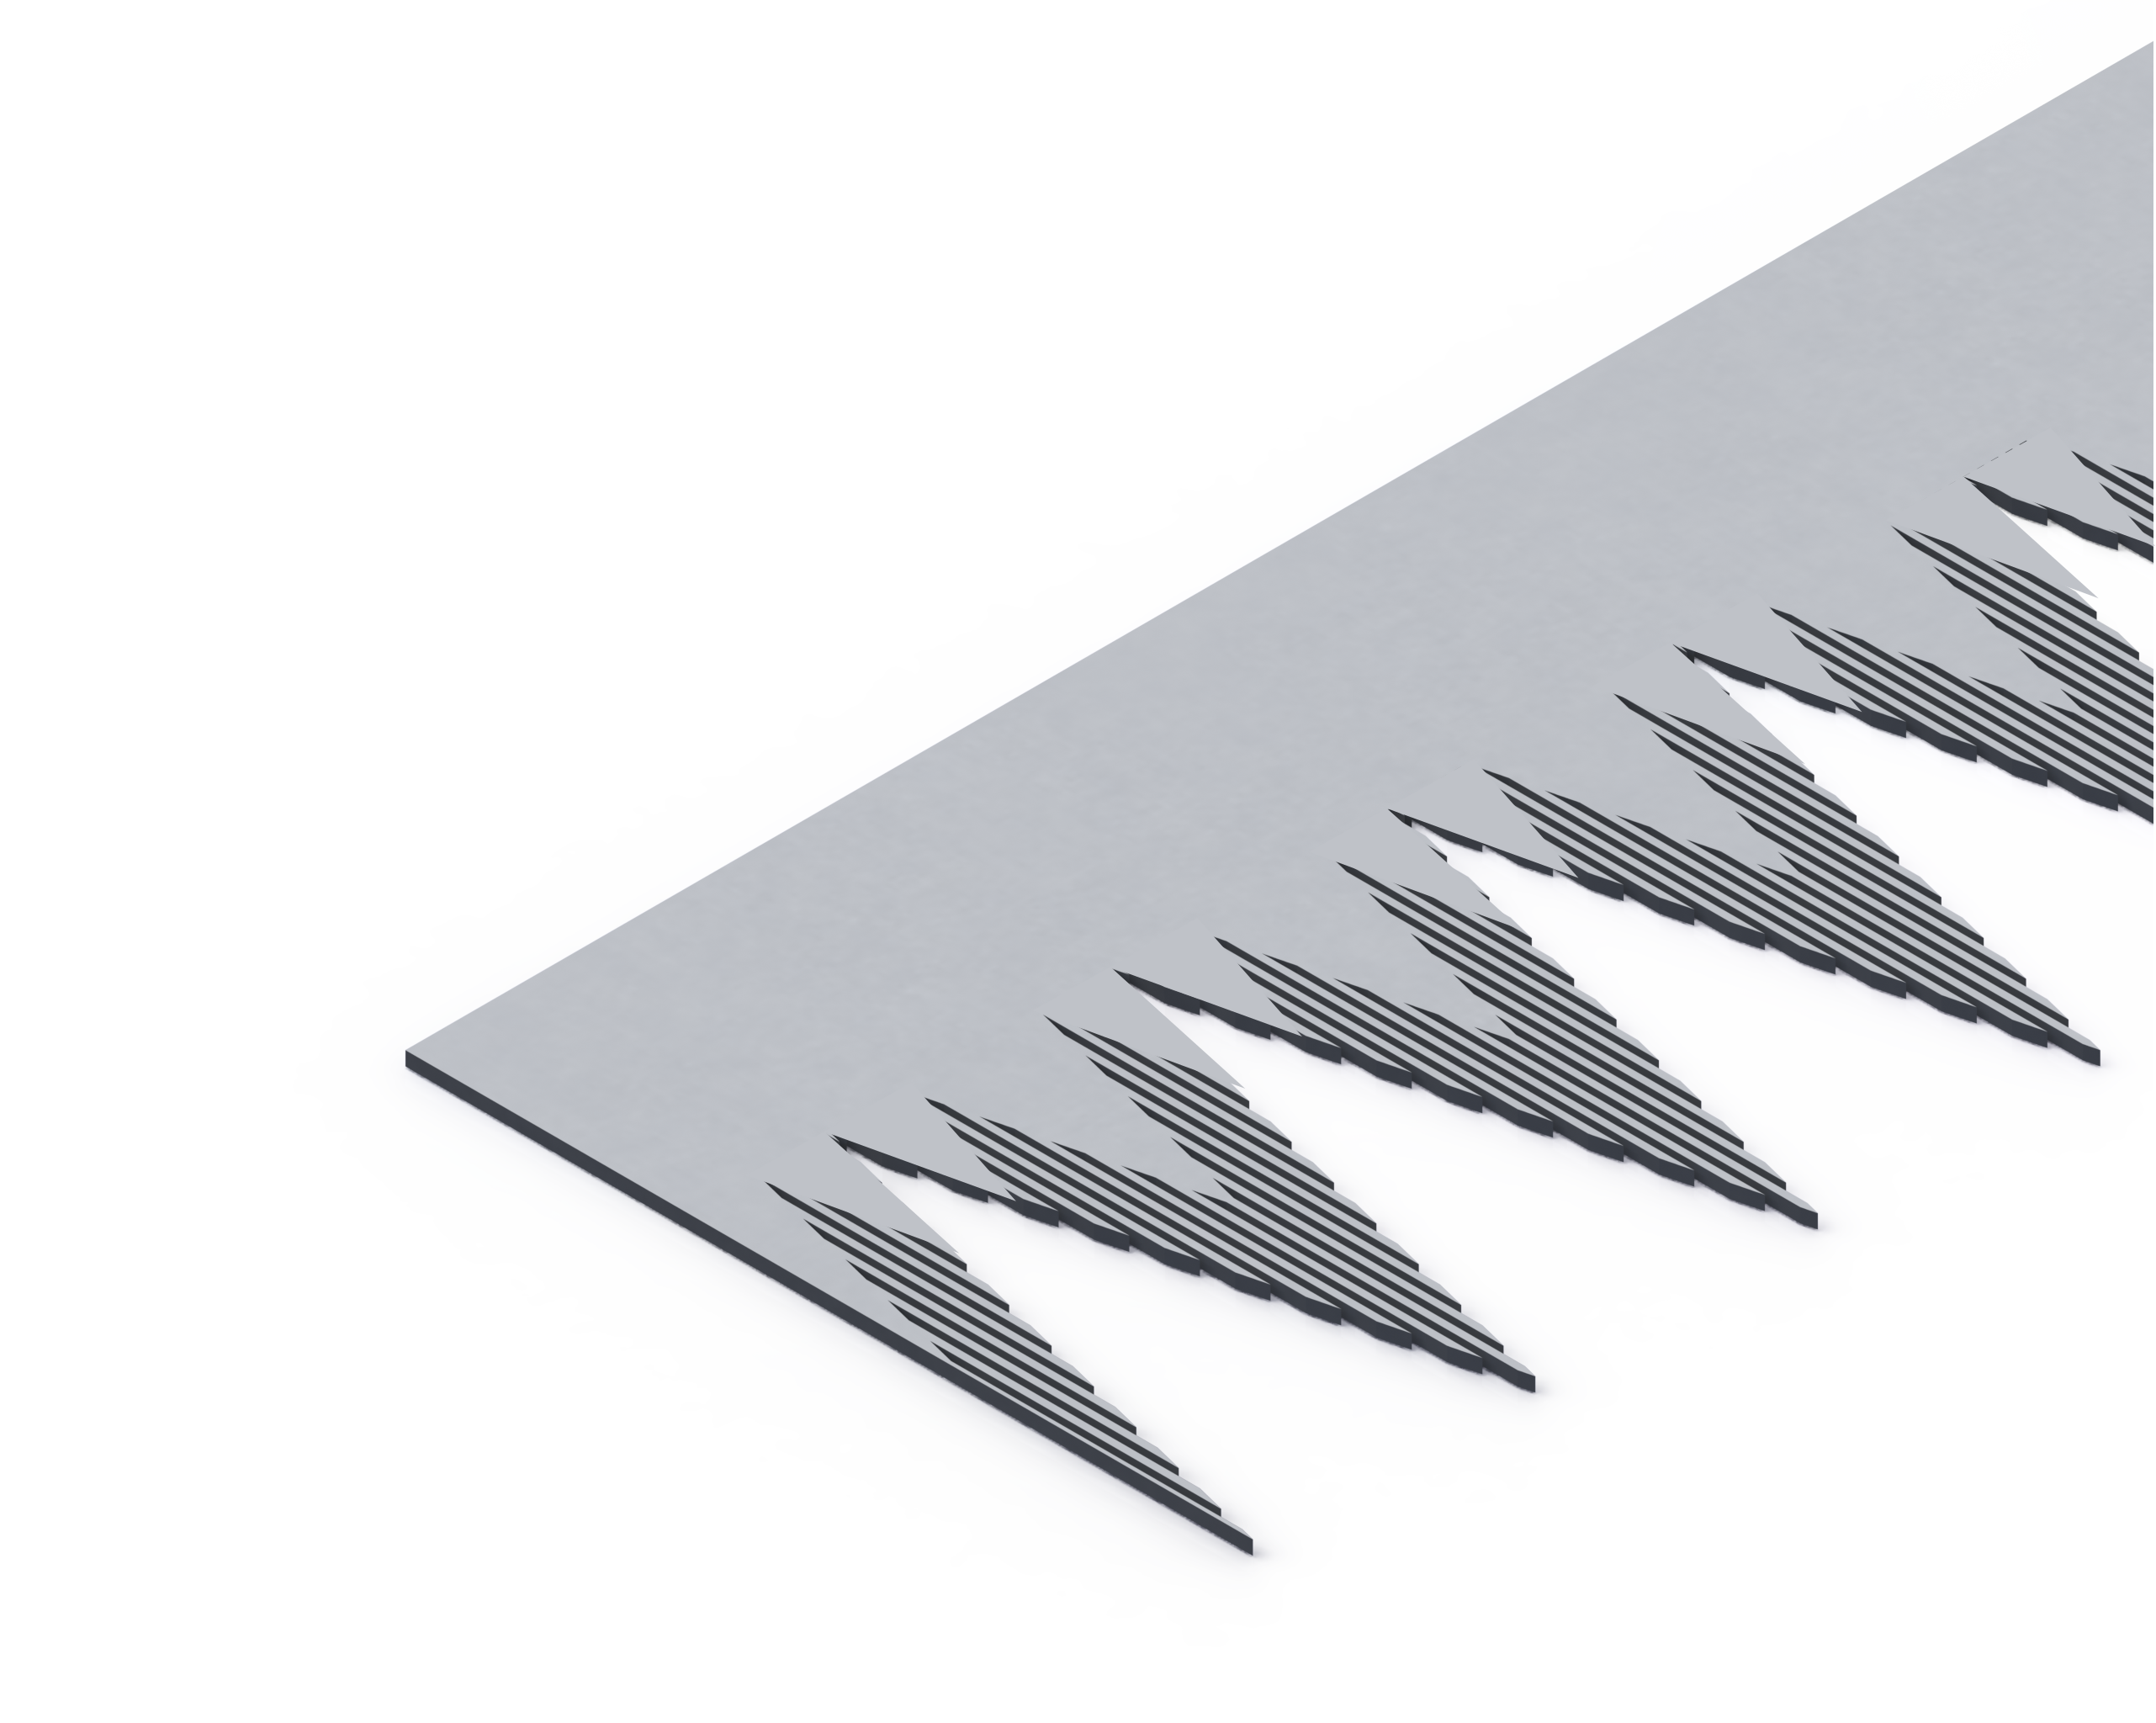
\includegraphics[width=0.9\textwidth]{media/Hybrids.png}}
    \end{columns}
\end{frame}

%This command inserts the ``Thank you for your attention''/Contact information
%slide with the information that was provided before about the owner information
\ClosePresentation

\section{References}
\renewcommand*{\bibfont}{\tiny}
\begin{frame}[allowframebreaks]
    \frametitle{References}
    \tiny{\bibliographystyle{plainnat}}
    \bibliography{/home/caar/Documents/Dropbox/PhD/bib/PhD.bib}
\end{frame}

\end{document}

